%%!TeX program = xelatex
%% 부득이하게 pdflatex을 사용해야 할 경우 위의 magic comment를 제거하십시오.

% Initiated by 정민석(2014년도 경기과학고 수학과전문교원)
% Continously being modified by 경기과학고 TeX 사용자협회
% Website : http://gshslatexintro.github.io 
% 과학전람회 양식에 맞추어 수정하였음.
\documentclass{junlam_reportK}
% 아래의 함수를 사용하면 이미지 파일들을 같은 디렉토리 내에 images 라는 이름을 가진 폴더를 생성한 후, 그 폴더 안에 넣어 사용할 수 있습니다.
% 사용하고자 한다면 주석을 푸십시오.
\graphicspath{{images/}}
% 이곳에 필요한 별도의 패키지들을 적어넣으시오.
%\usepackage{...}
\usepackage{verbatim} % for commment, verbatim environment
\usepackage{spverbatim} % automatic linebreak verbatim environment
%\usepacakge{indentfirst}
\usepackage{tikz}
%\tikzset{
%	image label/.style={
%		every node/.style={
			%fill=black,
			%text=white,
%			font=\sffamily\scriptsize,
%			anchor=south west,
%			xshift=0,
%			yshift=0,
%			at={(0,0)}
%		}
%	}
%}
\usepackage{amsmath}
\usepackage{amsfonts}
\usepackage{amssymb}
\usepackage{algorithm}
\usepackage{algpseudocode}
\usepackage{float}
\usepackage{graphicx}
\usepackage{tabularx}
\usepackage{multirow}
\usepackage{multicol}
% \setlength{\columnseprule}{0.5pt}
% \def\columnseprulecolor{\color{black}}


\usepackage{booktabs}
\usepackage{longtable}
\usepackage{gensymb}
\usepackage{wrapfig}
%\usepackage{subcaption}
%\usepackage{floatrow}
%\usepackage{pict2e}
%\usepackage[backend=biber,style=authoryear]{biblatex}
%\usepackage{biblatex}
\usepackage{pgfplots}
\pgfplotsset{
	compat=newest,
	label style={font=\sffamily\scriptsize},
	ticklabel style={font=\sffamily\scriptsize},
	legend style={font=\sffamily\tiny},
	major tick length=0.1cm,
	minor tick length=0.05cm,
	every x tick/.style={black},
}

\usetikzlibrary{shapes}
\usetikzlibrary{plotmarks}
\usepackage{listings}
\usepackage{hologo}
\usepackage{makecell}
\usepackage{color}
\lstset{
	basicstyle=\small\ttfamily,
	columns=flexible,
	breaklines=true
}

\citation
\bibdata

%: ----------------------------------------------------------------------
%:               보고서 정보를 입력하시오
% ----------------------------------------------------------------------
% 아래와 같은 command를 만들면 길이가 긴 용어를 간편하게 사용할 수 있습니다. 단, 이미 지정된 함수명들은 새로운 함수명으로 사용할 수 없습니다.
% 연, 월, 일은 보고서 제출 날짜에 맞게 수정하십시오.

% 출품학생
\studentnames{남도현, 백효송, 이시현} % 

% 지도교사
\advisor{박기현} % 

% 출품 번호
\summitnumber{지-6} % 

% 제출일과 과학전람회 회수
\summitdate{2023}{9}{2} % (연, 월, 일)
\junlam{69} % 과학전람회 회수 = 연도 - 1954 (ex. 2020년은 66회 대회)

% 출품 분야
\entryfield{학생} % 학생 / 교원

% 출품 부문
\entrysection{지구 및 환경} % 물리 / 화학 / 생물 / 산업 및 에너지 / 지구 및 환경

% 제목
% \title{확장 가능한 2차원 미니 조파 수조 제작 및 이를 활용한 연안 환경 모형 실험} % 제목 개행 시 \linebreak 사용. \\나 \newline 은 안됨.
\title{연안 환경 모형 실험을 위한 $2$차원 조파 수조 제작} % 제목 개행 

\newtheorem{definition}{정의}

 % usepackage 등의 명령어는 여기에.
\usepackage{cite}
\usepackage{textcomp}
\usepackage{tocloft}
\usepackage[utf8]{inputenc}
\usepackage[T1]{fontenc}
\usepackage[utf8]{inputenc}
\usepackage{lmodern}

\usepackage{minted}
\setlength{\cftbeforesecskip}{0pt}
\setlength{\cftbeforesubsecskip}{0pt}
\setlength{\cftbeforesubsubsecskip}{0pt}

% 본문 시작
\begin{document}
	%표지만들기
	%makecover 함수와 관련하여 "Underfull \hbox (badness 10000) in paragraph" 오류는 무시하십시오. (TeXstudio ver 2.9.4 오류 기준)
	%\makecover
	%\baselineskip=2.2em         % line spacing in the paragraph
	%\maketitle  % command to print the title page with above variables
\makecover  % command to print the title page with above variables

\setcounter{page}{1}
\renewcommand{\thepage}{\roman{page}}

%----------------------------------------------
%   Table of Contents (자동 작성됨)
%----------------------------------------------
\cleardoublepage
\addcontentsline{toc}{section}{Contents}
\setcounter{secnumdepth}{3} % organisational level that receives a numbers
\setcounter{tocdepth}{3}    % print table of contents for level 3
\baselineskip=2.2em
\tableofcontents


%----------------------------------------------
%     List of Figures/Tables (자동 작성됨)
%----------------------------------------------
\cleardoublepage
\clearpage
\listoffigures	% 그림 목록과 캡션을 출력한다. 만약 논문에 그림이 없다면 이 줄의 맨 앞에 %기호를 넣어서 코멘트 처리한다.

\cleardoublepage
\clearpage
\listoftables  % 표 목록과 캡션을 출력한다. 만약 논문에 표가 없다면 이 줄의 맨 앞에 %기호를 넣어서 코멘트 처리한다.


\cleardoublepage
\clearpage

%---------------------------------------------------------------------
%                  영문 초록을 입력하시오
%---------------------------------------------------------------------
%\begin{abstracts}     %this creates the heading for the abstract page
%	\addcontentsline{toc}{section}{Abstract}  %%% TOC에 표시
%	\noindent{
%			Put your abstract here. Once upon a time, \gshs said : `The first, and the best.'
%	}
%\end{abstracts}

%\cleardoublepage
%\clearpage

\begin{abstractskor}
	\addcontentsline{toc}{section}{초록}  %%% TOC에 표시
	\noindent{
		
	%본 연구에서는 해안, 연안 등을 소규모로 재현하여 연안 공학, 선박 공학 등과 관련된 모형 실험을 할 수 있는 2차원 조파 수조를 제작하였다. 조파 수조는 수조를 기본으로 하여 조파기, 소파기, 파고계, 해안 경사 등의 부분으로 구성되어 있다. 수조는 길이 $2,000~\mathrm{mm}$, 폭 $300~\mathrm{mm}$, 높이 $400~\mathrm{mm}$인 수조 모듈로 구성되어 있으며 3개를 연결하여 총 길이 $6,000~\mathrm{mm}$로 제작되었고 모듈을 추가하여 확장할 수 있다. 조파기는 리니어 엑츄에이터의 스텝 모터를 틴지 보드 기반의 컨트롤러로 제어하여 아두이노 코드로 여러 종류의 파를 만들어 낼 수 있어 다양한 모형 실험을 구현할 수 있다. 제작된 조파수조는 쓰나미에 의한 피해, 파력 발전의 효율, 효과 적인 방파제, 선박의 안정성 등을 알아보는 모형 실험에 적용할 수 있을 것으로 생각된다. 
    기후 위기의 심화로 연안 지형이 쓰나미, 태풍 등 자연재해에 대해 가장 큰 피해를 받고 있다. 이에 대처할 공법을 실험하기 위해서는 연안 모형을 조성할 수 있는 조파 수조가 필요하다. 본 연구에서는 연안을 소규모로 재현할 수 있는 2차원 조파 수조를 제작하였다. 조파 수조는 길이 $2,000~\mathrm{mm}$, 폭 $300~\mathrm{mm}$, 높이 $400~\mathrm{mm}$인 모듈 3개가 연결된 것을 기본 구조로 하며, 모듈을 추가 제작하여 연결해 길이를 연장할 수 있다. 수조를 기본으로 하여 조파기, 소파기, 파고계, 경사 모형으로 구성되어 있으며, 경사 모형은 탈부착이 가능하다. 조파기는 리니어 엑츄에이터의 스텝 모터를 틴지 보드 기반의 컨트롤러로 제어하는 방식으로 구동되며, 아두이노 코드로 여러 파를 제작할 수 있다. $\sin$파의 진동수를 지정할 수 있으며, 파고는 입력값과 완전히 일치하지 않으나, 실험을 통해 입력값과 출력값의 관계를 파악하여 원하는 파고를 근사하게 만들어낼 수 있다. 제작한 조파 수조를 방파제의 조적 구조 성능 비교, 파력 발전 모형 효율 축정, 쓰나미에 의한 구조물 피해 파악 실험 등에 사용할 수 있다. 
	}
\end{abstractskor}

 % Abstract
	
	%%%%%%%%%%%%%%%%%%%%%%%%%%%%%%%%%%%%%%%%%%%%%%%%%%%%%%%%%%%
	%%%% Main Document %%%%%%%%%%%%%%%%%%%%%%%%%%%%%%%%%%%%%%%%
	%%%%%%%%%%%%%%%%%%%%%%%%%%%%%%%%%%%%%%%%%%%%%%%%%%%%%%%%%%%
	\cleardoublepage
	\clearpage
	\renewcommand{\thepage}{\arabic{page}}
	\setcounter{page}{1}
	
	%각 장을 아래와 같이 sub 폴더 안에 만들어서 넣으면 편리하다.
	\section{서론}
%\section{Introduction}


\subsection{제작 동기}

방파제 조적 구조에 의한 방파 효과를 분석, 비교하는 연구를 계획하던 중 모형 실험을 위하여 연안 모형과 이곳에 해파를 발생시키는 장치가 필요하게 되었다. 선행 연구를 조사해 보니 연안 등 다양한 조건에서 해양 현상의 모의 실험은 조파 수조를 이용하여 할 수 있다는 것을 알게 되었다\cite{chung2013}. 해양환경관리공단(KOEM)은 해양환경개발교육원 내에 세계 최초로 인공해안이 설치된 조파 수조를 설치하고 발명 특허를 내기도 하였다 (등록번호 제10-0978231호). 또, KITECH 해양로봇센터, CIIZ, KIOST 한국해양과학기술원 등 다양한 기관에서는 대규모 조파 시설을 구비하여 타 기관이나 업체에서 시험을 의뢰받기도 한다. 본교에서도 해양 관련 연구가 자주 이뤄지기에 다양한 실험을 시행하기 위해서 조파 수조가 필요하지만 이는 시중에서 구하기 어려우며 상당히 고가이다. 이에 여러 해안 환경 모형 실험을 할 수 있는 조파 수조(wave flume)와 맞춤형 파를 제작할 수 있는 조파기(wave maker)를 제작하기로 하였다. 


\subsection{제작 목적}

본 조파 수조는 파도를 발생시카거나 이를 이용한 모형 실험을 하기 위하여 개발되었다. 조파 수조는 조파기, 소파기, 파고계, 연안 모형 등의 관련 시설을 포함하여 아래와 같은 모형 실험을 할 수 있도록 하는데 주된 목적이 있다.

\begin{enumerate}
    \item 쓰나미에 의한 피해를 알아보는 연안의 구조물 모형 실험
    \item 다양한 파력발전 모형 실험
    \item 방파제의 조적구조 효율 비교 실험
    \item 선박, 부표 등의 안정성 비교 실험
\end{enumerate}

본 연구에서는 2차원 조파수조를 제작하고 이를 이용하여 다양한 실험을 할 수 있도록 조파기의 성능을 검증하였다. 
 % 서론
	\section{이론적 배경}
%\section{Theoretical Background}

\subsection{조파 수조와 조파기}
조파 수조는 조파기가 달린 모형 실험용 수조로 해안 혹은 연안에서의 여러 현상을 축소하여 재현 및 실험하기 위한 장치이다. 정밀한 실험을 위해서 기업체나 연구실에서는 큰 스케일로 제작하기도 한다. 주로 선박의 안정성이나 연안에 설치한 구조물의 내구성 등을 시험할 때 맞는 환경을 조성해준다. 초기에는 실험적으로 만들어졌으나 유체 관련 연구가 진행되면서 이론적인 분석이 추가되었다. 
%본교에서 제작한 조파 수조는 파의 진행방향이 한 방향이며 2차원 조파 수조라고 부른다. 

소규모로 운영이 용이하며 비교적 정확한 파를 생성하고 변화를 관찰하기 위해서는 파의 진행방향이 한 방향인 2차원 조파 수조가 적합하다. 2차원 조파 수조를 이용하여 파 특성에 관한 기본 연구나 파와 물체 간의 상호작용에 대한 실험 연구를 충분히 수행할 수 있다. 

\begin{figure}[htbp]
\begin{center}
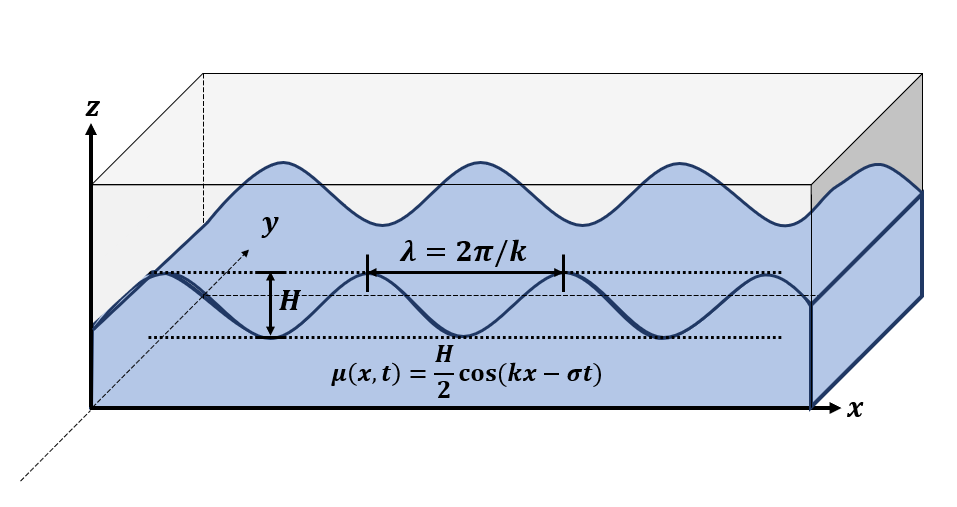
\includegraphics[width=10cm, trim={0 1.8cm 0 1.5cm}, clip]{Water_Tank(Illustrated).png}
\end{center}
\caption{조파 수조 모식도}
\label{Fig01}
\end{figure}
%해파를 만들때 현상을 재현하기 위한 환경을 조성하며 
조파기는 조파 수조에서 파를 생성하는 장치이다. 조파기는 판의 운동 방식에 따라 플랩형, 피스톤형, 플런저형 등이 있다. 피스톤형 조파기는 연안 환경에서의 실험에 자주 사용되는 천해파를 생성하기 용이하다. 피스톤형 조파기에서 파를 생성하는 조파판의 모든 요소는 일관적으로 수평 운동을 한다. 또, 판의 수평 운동 범위를 스트로크라고 하며 $S_0$로 쓰도록 한다 (단, 이는 판의 각 부분이 모두 함께 운동하는 경우에 해당한다).

% 세 종류의 조파기를 보여주는 그림이 필요함.
\begin{figure}[H]
    \begin{center}
        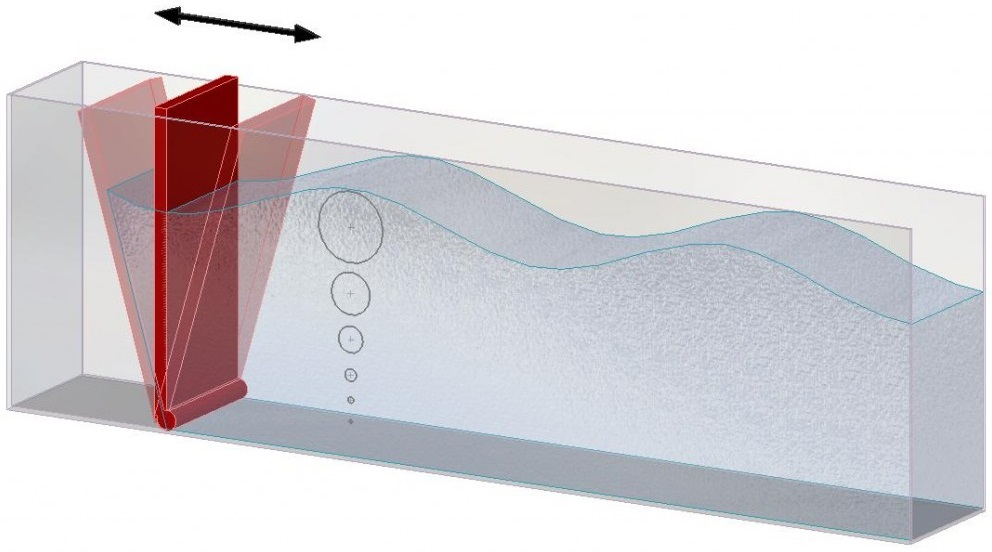
\includegraphics[height=3cm]{images/Wave_Maker(Flap).jpg}
        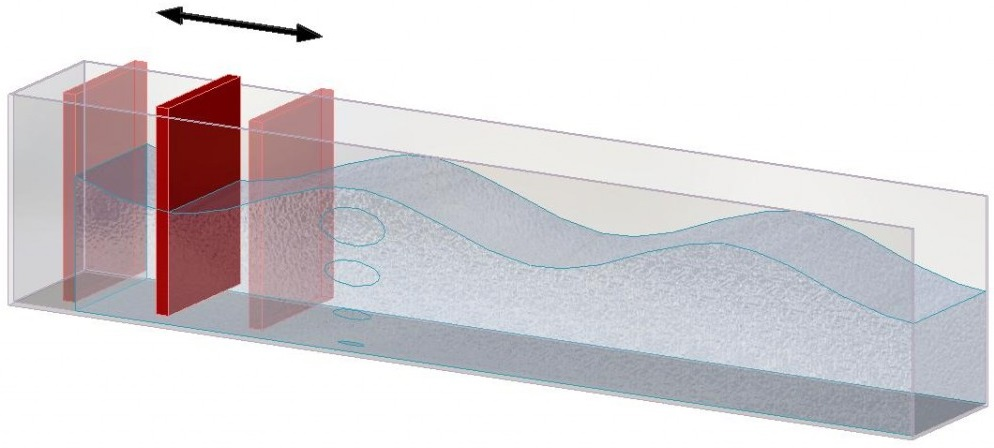
\includegraphics[height=3cm]{images/Wave_Maker(Piston).jpg}
    \end{center}
        \begin{tikzpicture} [remember picture, overlay]
            \node at (1.7, 1.0) {\scriptsize{(a) flap type}};
            \node at (7.6, 1.0) {\scriptsize{(b) piston type}};
        \end{tikzpicture}
        \caption{Various types of 2-dimensional wavemaker - (a) flap type (b) piston type}
        \label{Experimnet_System} 
\end{figure}

\subsection{조파 이론(wave maker theory)}

조파 이론은 여러 종류의 조파기가 발생하는 파도의 특성과 개형을 알아보는 것을 목표로 한다\cite{dean1991water} \cite{zhang2007deterministic} \cite{ojk2018}.
2차원 조파 수조에서 피스톤형 조파기가 발생시키는 파도는 여러 방정식을 통해 구할 수 있다. 제일 보편적인 방식은 속도 퍼텐셜 $\phi(x, y, z, t)$를 정의하고 이에 대한 라플라스 방정식과 여러 경계조건을 적용하는 것이다. 방정식을 풀면 속도 퍼텐셜은 다음과 같이 정해진다.

\begin{equation} \label{eq:1}
{
\phi(x, z, t) = A\cosh{[k(h+z)]}\sin(kx-\sigma t) +
\cos(\sigma t){\sum_{n=1}^{\infty}} C_n e^{-k_3 x} \cos{[k_3 (z+h)]} 
}
\end{equation}

%$$\phi(x, z, t) = A\cosh{[k(h+z)]}\sin(kx-\sigma t) + $$
%$$\cos(\sigma t){\sum_{n=1}^{\infty}} C_n e^{-k_3 x} \cos{[k_3 (z+h)]}  $$

파동은 $x$방향으로 진행하며 $h$는 수심이고 $k$는 파수, $\sigma$는 각진동수이다. 그외의 문자는 상수이며 식(\ref{eq:1})로부터 발생파의 변위 식을 다음과 같이 쓸 수 있다.

\begin{equation} \label{eq:2}
{
\mu(x, t) = {{1 \over g}{{\partial \phi} \over {\partial t}}|_{z=0} } = \frac{A \sigma}{g} \cosh(kh) \cos(kx-\sigma t) +
\sin(\sigma t) {\sum_{n=1}^{\infty}} \frac{\sigma C_n}{g} e^{-k_3 x} \cos(k_3 h)
}
\end{equation}

%$$\mu(x, t) = \frac{A \sigma}{g} \cosh(kh) \cos(kx-\sigma t) + $$
%$$\sin(\sigma t) {\sum_{n=1}^{\infty}} \frac{\sigma C_n}{g} e^{-k_3 x} cos(k_3 h) $$

식 (\ref{eq:1}), (\ref{eq:2}) 모두 첫 항은 진행파, 두 번째 항은 정상파를 의미한다. 정상파의 $k_3$은 진팽파의 분산관계식을 정상파 파수로 변환한 식에서 구할 수 있으며 $\sigma ^2 = -g k_3 \tan{k_3 h}$의 해이다. 하지만 제일 큰 해에 대해서 감쇠되는 비율 $\exp{(-k_{3}x)}$가 $x=2h$일 때 $0.04$, $x=3h$일 때 0.009 수준으로 급감하며 본 연구에서는 수조 길이가 6$m$, 수심이 약 15$cm$ 수준이므로 정상파는 무시할 수 있다. 또, 미분방정식의 각각의 고유함수에 대해 일차 근사를 적용하여 파고 $H$를 다음과 같이 표현할 수 있다.

\begin{equation} \label{eq:4}
H = \frac{4 S_0 \sin h{kh}}{\sin h{2kh}+2kh} \left(\sin h{k[z_d - h]} - \sin h{k[z_u - h]}\right)
\end{equation}

%$$H = \frac{4 S_0 \sin h{kh}}{\sin h{2kh}+2kh} (\sin h{k[z_d - h]} - \sin h{k[z_u - h]}) $$

$z_d$는 조파판 하단의 깊이, $z_u$는 조파판 상단의 깊이이며 본 연구의 경우 조파판이 수심 전체에 걸쳐 존재하므로 $z_d = h$, $z_u = 0$이고 파고와 파동 함수는 다음과 같다.

\begin{equation} \label{eq:5}
{
    \frac{H}{S_0}=\frac{4 \sinh^2 k h}{\sinh 2kh + 2kh}
     = \frac{4 \sinh^2 z}{\sinh 2z+2 z}, ~z=kh
}
\end{equation}

\begin{equation} \label{eq:6}
{
    \mu(x, t)=\frac{H}{2} \cos (k x-\sigma t)
}
\end{equation}

%$$\frac{H}{S_0}=\frac{4 \sinh ^2 k h}{\sinh k h+2 k h}, \mu(x, t)=\frac{H}{2} \cos (k x-\sigma t)$$

$S_0,~h$는 구조적인 값이며 조절이 가능하다. 또, 파수 $k$와 각진동수 $\sigma$는 분산 관계식을 만족하므로 결론적으로는 $\sigma$와 $S_0$, $h$를 정하면 된다. 조파판 또한 sin형으로 움직이도록 경계조건으로 반영되었으며 이 경우 판의 진동 변위는 다음과 같다.

\begin{equation} \label{eq:7}
{
    x = {{S_0}\over2} \sin{\sigma t}
}
\end{equation}

하지만 이는 심해파의 경우이다. 여러 경계조건과 근사를 하기 위한 조건이며 심해파는 간단하게 $h/\lambda > 1/2$인 파를 의미하기도 한다. 이와 반대로 천해파는 $h/\lambda < 1/20$인 파를 의미하며 상대적으로 얕은 바다에서 생기며 파가 진행하면서 부서진다. 그렇기 때문에 이론적으로 파의 개형을 해석적으로 유도하기는 거의 불가능하며 대부분의 선행연구는 섭동이론을 적용하거나 2차까지 근사를 하는 등 비선형으로 방정식을 수치해석한다\cite{society1993laboratory}. 

\subsection{소파 장치(wave absorber)}
파는 수조 내부에서 전달되며 진행파와 주변 장애물에 부딫혀 반사된 반사파로 나뉜다. 중첩의 원리에 의하여 수면파는 진행파와 반사에 의한 정상파의 선형 결합으로 표현되며 정상파가 주요 오차의 원인이 된다. 소파기는 반사파가 생기지 않도록 해주는 장치로 능동형 소파 장치(active wave absorber)\와 수동형 소파 장치(passive wave absorber)로 나뉜다\cite{ouellet1986survey}.

%\subsubsection{능동형 소파기}

능동형 소파 장치는 또 다른 조파기가 있어서 벽에 입사하는 파를 완전히 상쇄시킬 수 있는 파를 만들어 반사하지 않도록 하는 것이다. 벽에 입사하는 파의 개형을 실시간으로 측정하여 이에 맞는 파를 발생시킬 수 있어야 하며 상당히 고가의 장비이고 사용가능한 환경, 구조가 제한되어 있다. 이는 벽 부근에 다른 조파기를 설치하는 방식이며 파를 발생하는 조파기가 자체적으로 운동을 제어하여 반사파를 상쇄시키도록 움직일 수도 있다. 이는 '흡수 조파' 방식으로 조파판에서 파의 개형을 측정하여 반사파를 상쇄하는 파를 추가적으로 생성하는 것이다.

%\subsubsection{수동형 소파기(passive wave absorber)}

수동형 소파 장치는 추가적인 구조물을 설치하여 반사파의 에너지를 최소화하는 것을 목적으로 한다. 능동형 소파 장치와 달리 아무리 최적화를 해도 반사파가 존재하며 horsehair, crushed rock 등 여러 구조가 있다. 특히, 파를 효과적으로 소멸시키기 위해 다공성 판을 이용하며 공극률에 따른 반사계수 비교 등 다공성 구조 관련 연구가 많으며 이미 그 효율성이 입증되었다\cite{lim2014optimum, o2017methods}. 또, 경사로를 이용하기도 하는데 이는 주로 3D 조파 수조에서 파를 관찰하려는 영역이 아닌 다른 부분에서 최대한 상쇄시키기 위함이다. 경사로는 위로 볼록한 포물면을 띄는 경우가 제일 반사계수가 낮음이 밝혀졌다. 본 연구에서는 수동형 소파기를 사용할 것이다.

\subsection{파고계(wave gauge)}

파고계는 파도의 높이(파고)를 재기 위한 측정 장치이다. 측정 방식에 따라 용량식, 저항식, 수압식, 초음파식 등여러 종류로 나뉘며 사용하는 장소의 규모, 정밀도에 따라 달라진다. 본 연구에서는 저항형 파고계를 사용하려고 하였으나 제대로 측정이 되지 않았다. 핵심원리는 물에 잠긴 와이어의 깊이에 따라서 전기전도도가 달라지고 저항이 바뀌는 점을 이용하여 전류값과 수심을 대응시키는 것이다. 하지만 실제로 실험을 해본 결과 수심이 $20\mathrm{~cm}$가 바뀔동안 전류가 $0.1\mathrm{~A}$가 바뀌었으며 이 값이 최소눈금이다. 전류 증폭을 시도해보았으나 회로가 버틸 수 있는 범위 내에서는 측정을 할 수 없으며 결국 부표를 띄우고 영상을 찍어 파도의 파고 데이터를 얻어내는 방식을 채택하였다.

\subsection{Froude 상사 법칙}
모형실험을 하는 경우 축척이 달라지면 물리적 특성이 바뀐다. 이때 무차원 수가 보존되어야 한다는 원리가 Froude 상사 법칙이며 보존되는 무차원 수를 Froude 수라고 한다.\cite{briggs2013basics, chakrabarti1994offshore} 이외에도 Reynolds 수, Prandtl 수 등이 보존되기도 하나 본 실험의 경우 액체의 점성이나 확산보다는 파의 진행에 초점을 맞추기 때문에 Froude 수가 보존되는 경우를 생각한다. Froude 수는 다음과 같이 정의된다.
\begin{equation}
    Fr = \frac{V}{\sqrt{gL}}
\end{equation}

$V$는 움직이는 개체(파도; 물, 배, 비행기 등)의 속도이며 $g$는 중력가속도, $L$은 계의 특성길이이다. 수조와 바다에 대한 Froude 수가 같아야 하며 두 계 모두 움직이는 개체는 파도이기 때문에 분산 관계식을 이용하여 새롭게 쓸 수 있다.

\begin{equation}
    Fr = \sqrt{\frac{\tanh{kh}}{kL}}
\end{equation}

특성 길이는 단면이 직사각형이 수조의 경우 $L = {2ab}/{(a+b)}$임이 알려져 있으며 $a$는 수조의 폭, $b$는 수조 내 물의 수심이다. 바다의 경우 이를 근사적으로 $2h$로 생각할 수 있다 ($h$는 바다의 수심이다). $a=30\mathrm{~cm}, b=15\mathrm{~cm}$를 대입하여 관계식을 구해보면 다음과 같다.

\begin{quote}
    \[f(z_i) = \frac{\tanh{z_i}}{z_i},~  z_i = k_i h_i\]

    \begin{multicols}{2}

    계 1: 수조
    \[{Fr_1}^{2} = \frac{a+b}{2ab} \frac{\tanh{k_1 b}}{k_1} = \frac{3}{4} f(z_{1})\]

    \columnbreak
    
    계 2: 깊은 바다
    \[{Fr_2}^{2} = \frac{1}{2h_2} \frac{\tanh{k_2 h_2}}{k_2} = \frac{1}{2} f(z_{2})\]
    \end{multicols}

\end{quote}

\begin{equation}
    \therefore \frac{3}{2}f(z_1 ) = f(z_2 )
\end{equation}

$z_i = 2\pi h_i/\lambda_i$이므로 심해파, 천해파의 경계값(각각 $h/\lambda = 1/2, 1/20$)을 대입해보면 모형 실험의 경우 천해파는 $\omega \sim \pi$이고 심해파는 $\omega \sim 4\pi$ 정도는 되어야 한다는 결론을 내릴 수 있다. 단, 이는 수조의 수심이 $15\mathrm{~cm}$인 경우이며 더 깊어져도 약 $20\mathrm{~cm}$정도가 최대이고 얕아진다고 한들 $\omega$는 각각 $\pi$, $4\pi$ 정도는 되어야 한다.




 % 이론적 배경
	\section{2차원 조파 수조 제작 결과}

\subsection{조파 수조 개관}

\begin{figure}[H]
        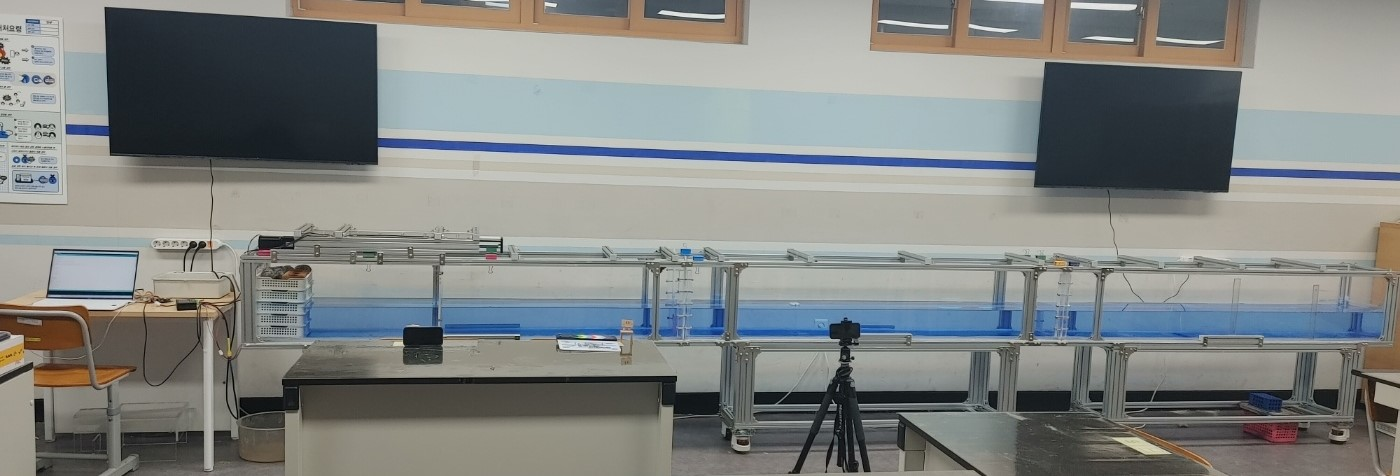
\includegraphics[width=\textwidth]{images/Experiment_System_Crop}
        \captionof{figure}{완성된 조파수조의 모습}
        
 %       \label{Experimnet_System} 
        \begin{tikzpicture} [remember picture, overlay, anchor=north west]
            \node [draw=yellow, text=yellow] (TV1) at (2.5, 5.8) {\scriptsize{TV1}};
            \node [draw=yellow, text=yellow] (TV2) at (14, 5.5) {\scriptsize{TV2}};
            \node [draw=yellow, text=yellow] (computer) at (1.0, 4) {\scriptsize{computer}};
            \node [draw=yellow, text=yellow] at (4.6, 2.6) {\scriptsize{camera1}};
            \node [draw=yellow, text=yellow] at (9.5, 2.5) {\scriptsize{camera2}}; 
        \end{tikzpicture}
        %\captionof{figure}{\scriptsize 완성된 조파 수조의 모습} %\\[0.5em]\
\end{figure}
 
제작한 작품은 '2차원 조파 수조'로 명명하였다. 이 조파 수조를 이용하여 실험을 할때 제대로 진행이 되려면 조파기, 소파기, 파고계, 해안 경사로 등이 제 역할을 해 주어야 가능하다. 따라서 각 부분은 실험 목적에 따라 조립과 분해가 가능하도록 따로 제작하였다. 제작한 조파 수조의 특징을 나열하면 다음과 같다.

\begin{itemize}
    \item 폭 $300~\mathrm{mm}$, 높이 $400~\mathrm{mm}$, 총 길이 $6,000~\mathrm{mm}$의 2차원 조파 수조를 제작하였다. 폭과 높이를 맞추어 수조 모듈을 추가로 제작하여 연결하면 얼마든지 길이를 확장할 수 있다. 
    \item 조파기는 리니어 엑츄레이터를 이용하여 구동부를 제작하였고 틴지 보드를 기반으로 하여 스텝 모터를 움직이는 제어부를 제작하였다. 
    \item 현재 조파기로 규칙파를 생성하는 코드를 완성하여 검증하고 있으며, 코드가 정교화되면 원하는 주기, 파장, 파고의 규칙파를 생성할 수 있다. 
    \item 이후 조파기는 쓰나미 등의 불규칙파를 생성할 수 있도록 정교한 제어를 할 수 있도록 코드를 업그레이드 할 예정이다. 
    \item 해안 경사로는 교각 위에 아크릴 판을 올리는 구조로 설계하여 길이와 기울기를 변화시켜 탈부착이 가능하도록 제작하였다. 
    \item 파고계는 물에 잘 뜨는 재질로 제작하여 동영상 분석을 통해 파고를 파악하고 있으며, 이후 센서를 부착하여 정밀한 파고를 측정하도록 개선할 예정이다.
\end{itemize}

\subsection{수조 모듈 구성 및 연결 방법}
수조는 길이 $2,000~\mathrm{mm}$, 폭 $300~\mathrm{mm}$, 높이 $400~\mathrm{mm}$인 수조 모듈로 구성되어 있으며 3개를 연결하여 총 길이 $6,000~\mathrm{mm}$이다. 수조 모듈의 기본 프레임은 알루미늄 프로파일로 제작하였으며 그 안에 두께 $5~\mathrm{mm}$의 아크릴 판을 이용하여 물이 담기는 수조를 제작하였다. 수조의 모서리 부분은 인접한 두 아크릴 판을 아크릴 접착제로 붙였으며 추가적으로 실리콘으로 방수 처리를 하였다. $2,000~\mathrm{mm}$ 길이의 수조 모듈을 서로 연결할 때는 물이 새지 않도록 매우 정교하게 붙여야 한다. 특히, 수준기로 수평이 맞는지 여러 방향에서 확인하여 모듈 3개가 일직선을 이루도록 해야 한다. 수조 모듈을 연결하는 연결부는 실리콘 패드를 잘라 모듈 사이에 끼웠고 아크릴 판의 옆, 아래에는 볼트가 들어갈만한 크기의 아크릴 조인트를 부착하여 볼트와 너트로 조이는 방법을 채택하였다. 수조 연결부도 실리콘으로 방수 처리를 하여 물이 새지 않는 총 길이 $6,000~\mathrm{mm}$의 수조를 완성하였다. 더 긴 수조가 필요하면 규격에 맞는 수조 모듈을 추가로 제작하여 사이에 끼워 붙여 길게 확장이이 가능하다.

\begin{figure}[h]
	\begin{center}
		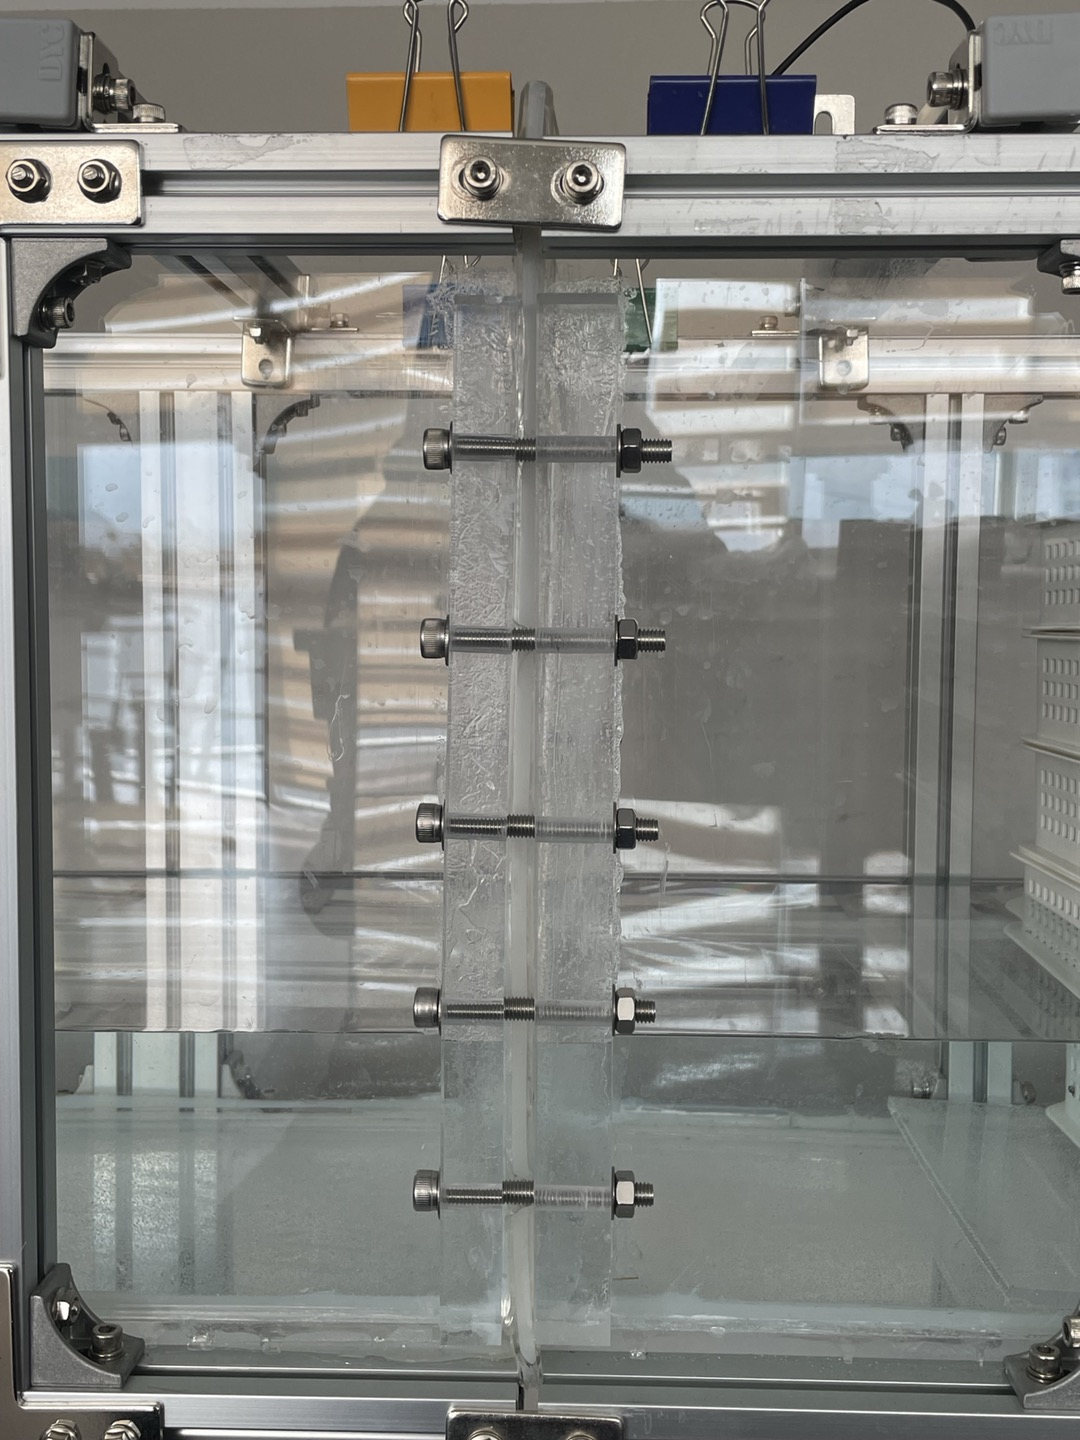
\includegraphics[width=0.3\textwidth]{images/magam1.jpg}
		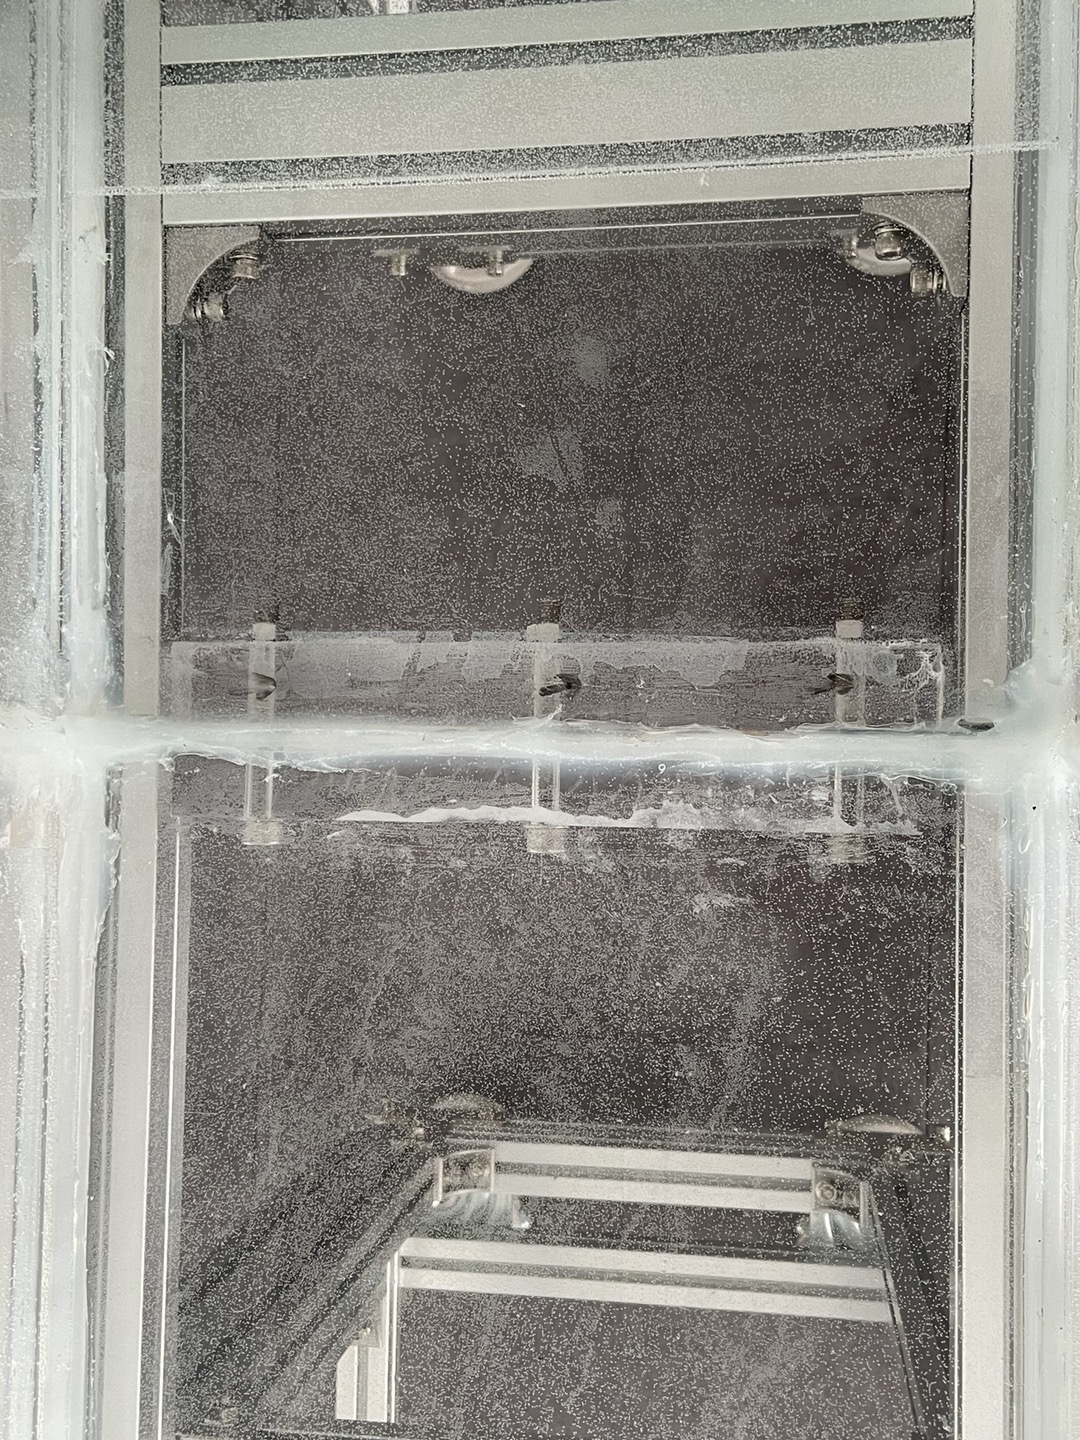
\includegraphics[width=0.3\textwidth]{images/magam2.jpg}
		\caption{수조 연결부의 모습}
		\label{Waveabsorber}
	\end{center}
\end{figure}

\subsection{소파 장치}
해파가 전파되다가 벽이나 장애물에 부딫히게 되면 반사파가 발생하는데, 수조는 양 끝이 막힌 구조로 되어 있어 조파기에서 출발한 해파와 반사파가 간섭을 일으키고 결과적으로 정상파가 만들어져 해파 실험에 지장을 준다. 대부분의 실험에서는 맞춤형 환경 조성을 위해 반사파를 상쇄시키는 소파 장치가 매우 중요하다.

조파판이 식 (\ref{eq:7})\을 따라 움직이면서 판의 뒷부분으로 진행하는 파도 생성한다. 판의 앞부분으로 진행하는 파는 수조의 말단에서 정상파를 형성하지만 $x/h > 20$이므로 (수심은 채 $30\mathrm{~cm}$가 되지 않는다.) 충분히 무시할 수 있다. 하지만 이는 수조가 무한히 길다고 가정한 상황이며 우리 수조의 경우 비록 $x/h > 20$이지만 반사파가 생길 수 있다. 또, 판의 뒷부분으로 진행하는 파는 상당히 좁은 공간에서 계속 중첩되므로 판에 계속해서 부하를 가하기 때문에 파를 소멸시킬 소파 장치가 필요하다.

\begin{figure}[h]
	\begin{center}
		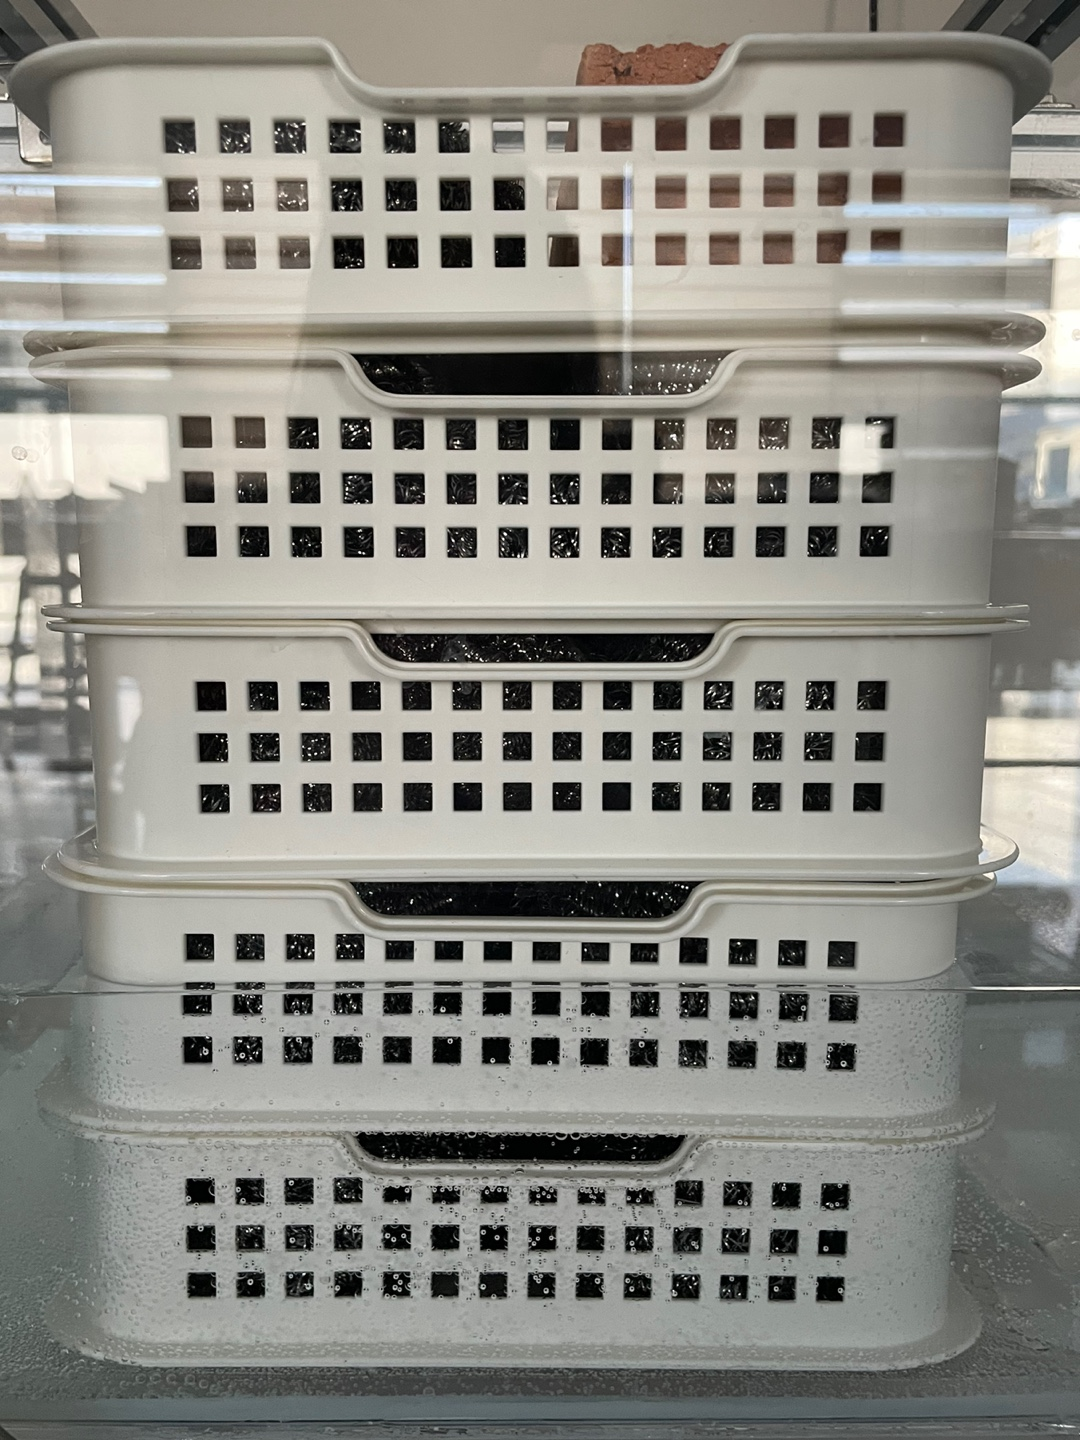
\includegraphics[width=0.3\textwidth]{images/sopagi1.jpg}
		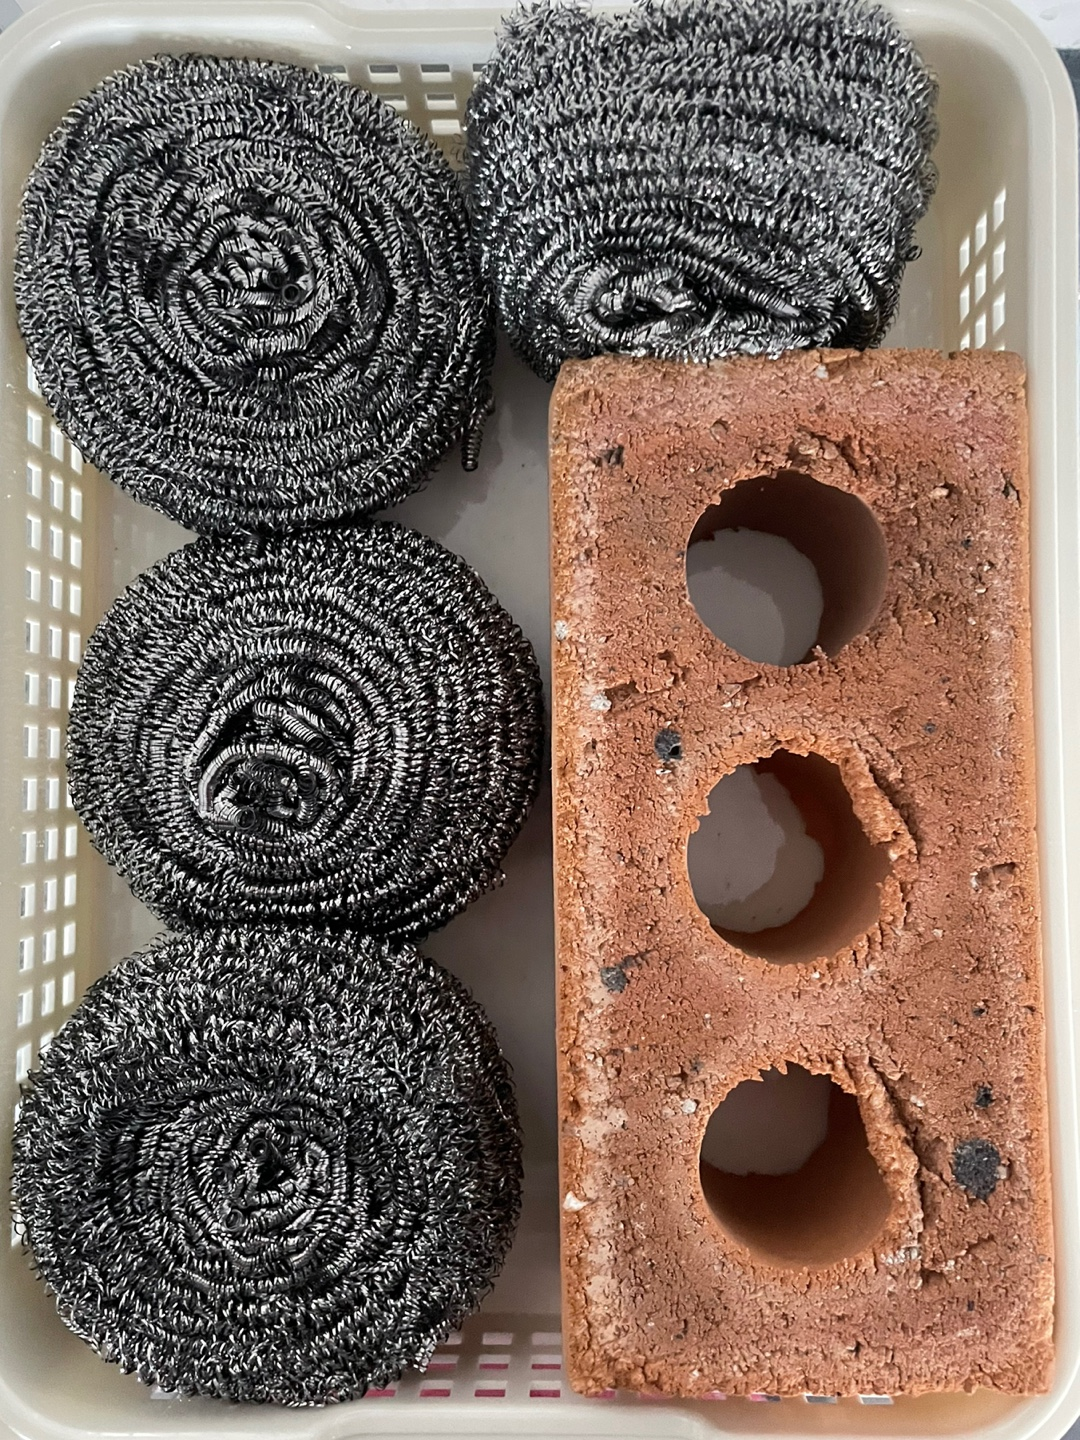
\includegraphics[width=0.3\textwidth]{images/sopagi2.jpg}
		\caption{플라스틱 바구니와 수세미를 이용해 만든 소파 장치}
		\label{Waveabsorber}
	\end{center}
\end{figure}

소파 장치는 해파의 에너지를 흡수할 수 있는 다공질의 구조가 소파 성능이 좋다는 점에 착안하여 구멍이 뚫린 플라스틱 바구니에 철 수세미를 넣는 방식으로 간단하게 제작하였다 \cite{lim2014optimum, o2017methods}. 플라스틱 바구니에 철수세미를 최대한 밀착하여 집어넣어 다공성 구조를 형성해주었고 소파 장치가 가벼워 파도에 의해 움직이기 때문에 이를 고정시키기 위해 가장 윗 칸에 벽돌을 올려 눌러주었다. 이렇게 2개를 만들어 조파 수조의 양 말단에 설치할 수 있도록 하였다. 

\subsection{연안 모형(해안 경사)}

먼 바다에서 해안으로 올수록 수심이 얕아지므로 해파는 심해파, 천이파, 천해파로 바뀌면서 바닥의 영향을 많이 받게 된다. 이 과정에서 파가 굴절하기도 하고, 속도가 느려지면서 쇄파 현상이 발생하게 된다. 해파는 연안의 모양에 따라 서로 다른 영향을 줄 수 있어 여러 연안 모형에 대해서 실험을 해야할 경우가 존재한다.

이러한 점을 감안하여 연안 모형은 목적에 맡게 바꿀 수 있고 탈부착이 가능하도록 설계하였다. 일정한 너비의 아크릴 판을 수조 바닥에 부착하고 육지 쪽은 높이 차를 만들기 위해 해안 경사 바닥을 안정적으로 지지할 수 있도록 알루미늄 프로파일 교각을 설치하였다. 실제 우리나라 주변의 바다만 하더라도 동해, 황해, 남해의 전형적인 해안 경사가 다르고, 해안 경사는 해파의 영향으로 항상 변할수 있기에 다양한 기울기의 해안 경사를 가질 수 있도록 해안 경사 바닥을 지지하는 교각의 길이를 다양하게 준비해 두었다. 현재 설치한 경사로는 높이 $200\mathrm{~mm}$, 길이 $2,000\mathrm{~mm}$로 기울기가 $1/10$ 이다. 

\begin{figure}[htbp]
	\begin{center}
		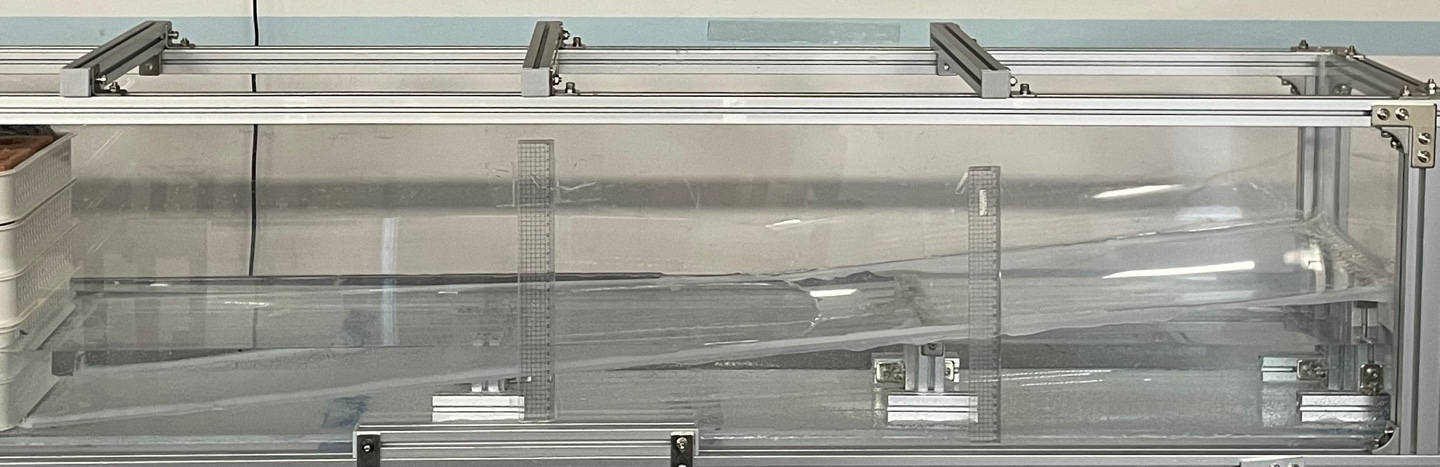
\includegraphics[width=0.8\textwidth]{images/slope.jpg}
		\caption{설치한 연안 모형}
		\label{Slope}
	\end{center}
\end{figure}


\subsection{방파제 모형}
현재 해안 모형은 경사로로 두었다. 하지만 경사로를 앞으로 이동시키고 뒷부분의 공간에 평지를 두면 구조물을 설치할 수 있다. 여기에 파력 발전 시설을 두어 여러 발전 시스템의 효율 비교 및 최적화 연구를 진행할 수도 있고 구조물의 내구성 실험을 할 수도 있다. 나아가 경사로의 경사로 변화시켜 여러 환경에서 다양한 실험을 진행할 수 있다. 또, 경사로를 받치는 부품이 녹슬었는데 이는 다른 재료로 대체하거나 경사로를 판을 덧대는 것이 아닌 일체형으로 만들어 관리가 쉽게 할 예정이다.

\begin{figure}[htbp]
    \centering
    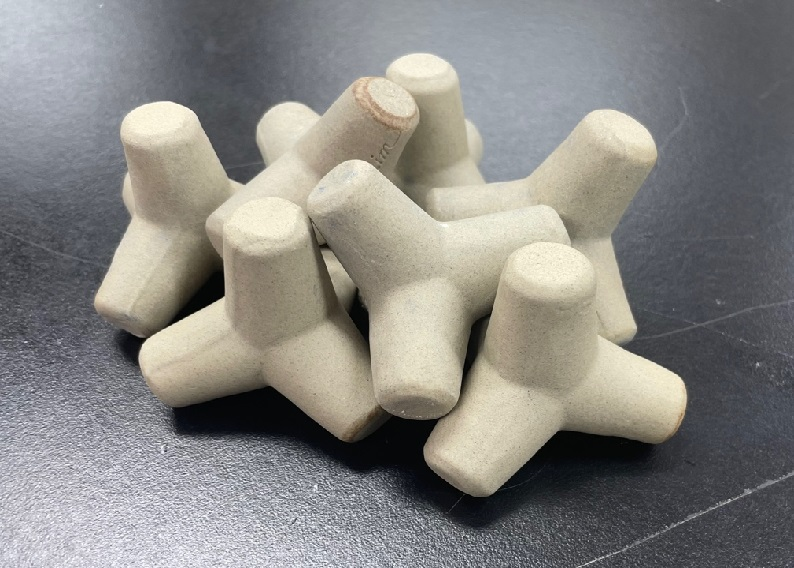
\includegraphics[height=5.5cm]{images/Breakwater.jpg}
    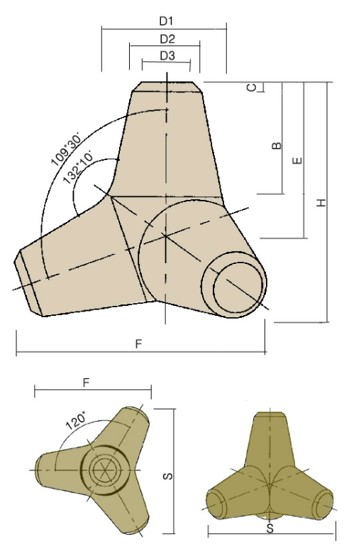
\includegraphics[height=5.5cm]{images/Breakwater(Illustrated).jpg}
    \caption{방파제 모형(왼쪽)과 규격(오른쪽)}
    \label{Braekwater}
\end{figure}

규격 $D3=1.2\mathrm{~cm}, D2=1.7\mathrm{~cm}, S=5.3\mathrm{~cm}, F=5\mathrm{~cm}$의 방파제 모형을 이용한 연구를 진행할 예정이다. 방파제의 조적 구조는 Gurer의 구조, Fabiao의 구조 등 여러 종류가 있으며 구조의 종류 및 스케일에 대한 방파 효과를 비교할 수도 있다\cite{article}.




\subsection{조파기}

%조파기 설계도를 넣어야 하는가? (넣는다면 다시 그릴 필요가 있음. 이전에 그렸던 것은 비율도 맞지 않고 전체적인 모습을 나타내지 못 함)

%조파기 사진
조파기는 구동부와 제어부로 나뉜다. 구동부는 조파기의 기계적인 부분으로 실질적인 움직임을 담당하며 리니어 액츄에이터와 이를 고정할 여러 부품으로 구성되어 있다. 제어부는 모터의 회전을 제어하는 부분으로 모터 드라이버와 틴지 보드 3.2(Teensy Board)로 구성되어 있다.

\subsubsection{구동부}
구동부는 $80\mathrm{~cm}$ 길이의 리니어 액츄에이터(linear actuator)를 메인 부품으로 하여 알루미늄 프로파일 프레임을 만들었다. 리니어 액츄에이터의 운동부에는 아크릴 재질의 조파판을 달았다. 조파판이 조파 수조 내부에 들어가도록 구동부를 수조 위에 설치하였다. 아크릴 판이 조파판이며 규격은 $280\mathrm{~mm} ~\times~ 295\mathrm{~mm} ~\times~5\mathrm{~mm}$로 수조 내부 공간에 딱 들어맞게 제작하였다. 조파판이 수조 내부의 벽과 최대한 밀착되어 있어야 정교한 파를 생성할 수 있다. 리니어 액츄에이터의 이동부에 붙어 수조 내부를 수평적으로 이동하며 물을 밀어내고 파를 생성한다. 액츄에이터는 FUYU 사의 FSK80 시리즈 제품으로 가동범위(stroke)는 $80\mathrm{~cm}$이고 최대 힘 $40\mathrm{~N}$, 최대 속력 $23\mathrm{~cm/s}$을 낼 수 있다(표 \ref{Specification of Linear Actuator}).

% \begin{figure}[H]
%     \begin{minipage}[t]{.3\linewidth}
%     \begin{center}
%         \scalebox{-1}[1]{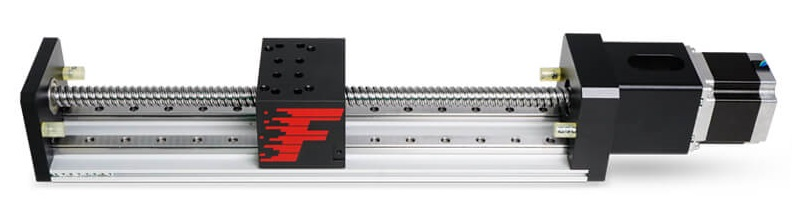
\includegraphics[width = 3cm]{images/Linear_Actuator.jpg}}
%         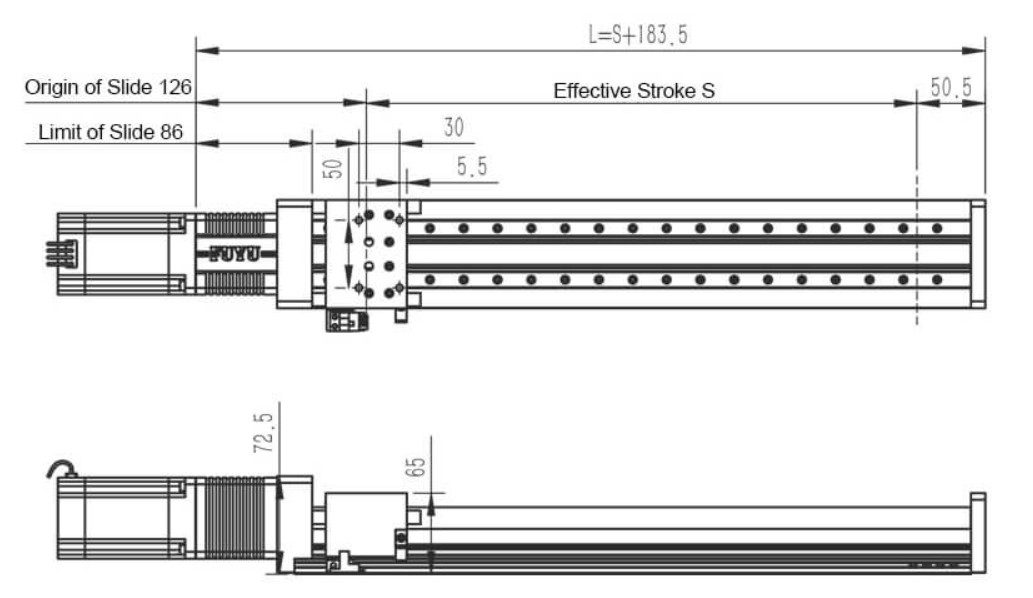
\includegraphics[width = 3cm]{images/Linear_Actuator(Design).jpg}
%     \end{center}
%         \begin{tikzpicture} [remember picture, overlay]
%         \node at (2.0, 11.0) {(a)};
%         \node at (2.0, 7.6) {(b)}; %1.1
%         \end{tikzpicture}	
%         %\caption{Linear actuator - (a) \textit{FSK80} series (b) Design}
%         \caption{(a) FUYU사의 FSK80 시리즈 리니어 액츄에이터, (b) 제원}
%         \label{linear actuator}
%     \centering
%   \end{minipage}\hfill
  
%   \begin{minipage}[t]{.6\linewidth}
%     \centering
%     \captionsetup{justification=centering}
%     \caption{리니어 액츄에이터의 스펙}
%     \begin{tabular}{l|l}
%         \hline
%         guide width $(\mathrm{mm})$                       & 80                                     \\
%         repeat position accuracy $(\mathrm{mm})$          & $\pm$0.02                                 \\
%         motor                                  & stepper 60102                          \\
%         % rail model                             & dual rail W12 $\times$ H8              \\
%         % ball screw model                       & 16                                     \\
%         \textbf{stroke $(\mathrm{mm})$}                  & \textbf{50 - 1000}                                    \\
%         pitch                                  & 10                                     \\
%         \textbf{horizontal full payload speed $(\mathrm{mm/s})$}   & \textbf{230}                                    \\
%         vertical full payload speed $(\mathrm{mm/s})$     & 60                                     \\
%         side mounting payload speed $(\mathrm{mm/s})$     & 210                                    \\
%         \textbf{rated horizontal payload $(\mathrm{kg})$}          & \textbf{40}                                     \\
%         rated vertical payload $(\mathrm{kg})$            & 20                                     \\
%         rated side mounting payload $(\mathrm{kg})$       & 15                                     \\
%         noisy without payload $(\mathrm{db})$             & 79                                     \\
%         rated payload noisy $(\mathrm{db})$               & 70                                     \\
%         \textbf{acceleration } $(\mathrm{mm/s}^{2})$   & \textbf{500}                                    \\ \hline
%     \end{tabular}%
%     \label{Specification of Linear Actuator}
%   \end{minipage}
% \end{figure}

%%%%%%%%%%%%%%%%%%%%%%%%%%%%%%%%%%%%%%%%%%%%%%%%%%%%%%%%%%%%%%%%%%%%%%%%%%%%%
\begin{figure}[H]
    \begin{center}
        \scalebox{-1}[1]{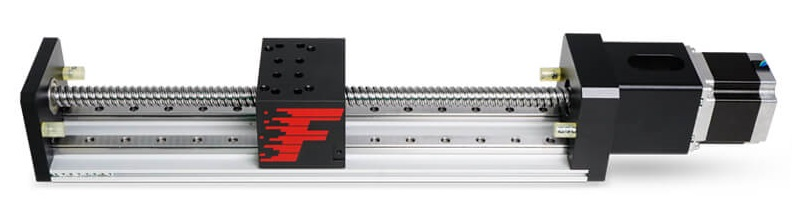
\includegraphics[width = 12cm]{images/Linear_Actuator.jpg}}
        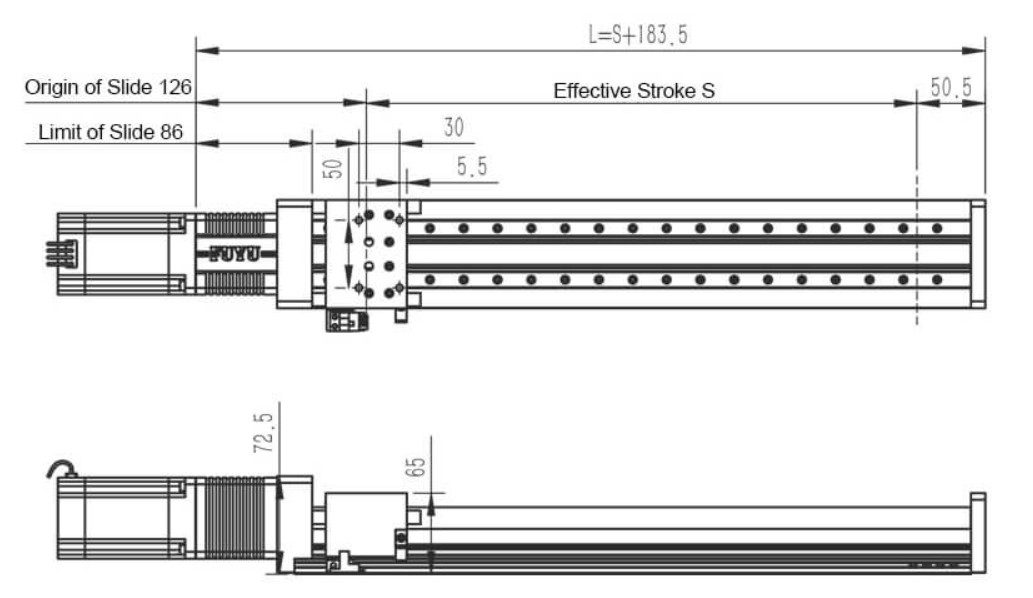
\includegraphics[width = 12cm]{images/Linear_Actuator(Design).jpg}
    \end{center}
        \begin{tikzpicture} [remember picture, overlay]
        \node at (2.0, 11.0) {(a)};
        \node at (2.0, 7.6) {(b)}; %1.1
        \end{tikzpicture}	
        %\caption{Linear actuator - (a) \textit{FSK80} series (b) Design}
        \caption{(a) FUYU사의 FSK80 시리즈 리니어 액츄에이터, (b) 제원}
        \label{linear actuator}
\end{figure}
%%%%%%%%%%%%%%%%%%%%%%%%%%%%%%%%%%%%%%%%%%%%%%%%%%%%%%%%%%%%%%%%%%%%%%%%%%%%

% \begin{figure}[H]
%     \centering
%     \captionsetup{justification=centering}
%     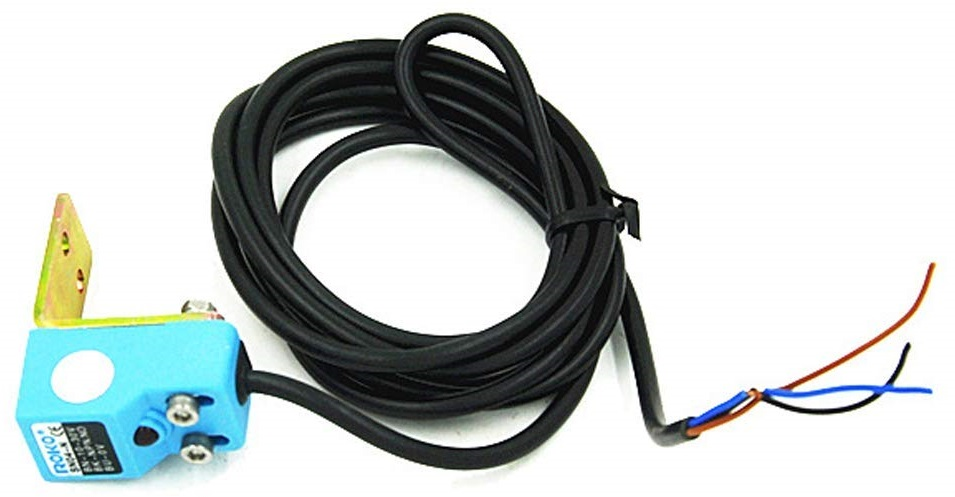
\includegraphics[width = 6cm]{images/Limit_Switch.jpg}
%     \caption{Limit Switch}
%     \label{limit switch}
% \end{figure}

% \begin{figure}
%     \centering
%     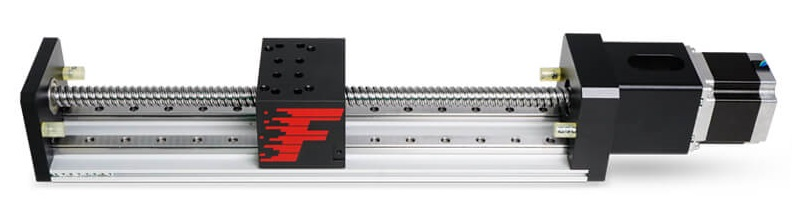
\includegraphics[width=0.5\textwidth]{images/Linear_Actuator.jpg}
%     \caption{FUYU사의 FSK80 시리즈 리니어 액츄에이터}
%     \label{Linear Actuator}
% \end{figure}

\begin{figure}
    \begin{minipage}[b]{.45\linewidth}
        \centering
        \scalebox{-1}[1]{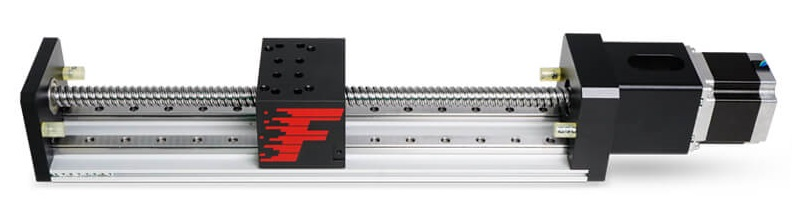
\includegraphics[width = 0.45\linewidth]{images/Linear_Actuator.jpg}}
        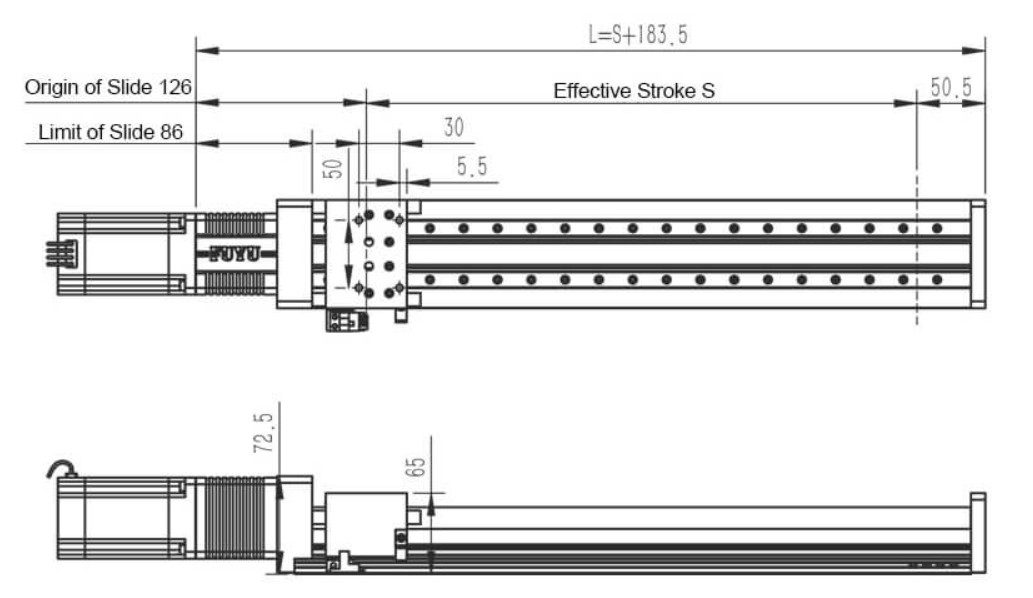
\includegraphics[width = 6cm]{images/Linear_Actuator(Design).jpg}
        % \begin{tikzpicture} [remember picture, overlay]
        %     \node at (2.0, 11.0) {(a)};
        %     \node at (2.0, 7.6) {(b)}; %1.1
        % \end{tikzpicture}	
        %\caption{Linear actuator - (a) \textit{FSK80} series (b) Design}
        \captionof{figure}{FUYU사의 FSK80 시리즈 리니어 액츄에이터}
        \label{linear actuator}
    \end{minipage}\hfill
    
    \begin{minipage}[b]{.45\linewidth}
        \resizebox{\columnwidth}{!}{
        \begin{tabular}{l|l}
            \hline
            guide width $(\mathrm{mm})$                       & 80                                     \\
            repeat position accuracy $(\mathrm{mm})$          & $\pm$0.02                                 \\
            motor                                  & stepper 60102                          \\
            % rail model                             & dual rail W12 $\times$ H8              \\
            % ball screw model                       & 16                                     \\
            \textbf{stroke $(\mathrm{mm})$}                  & \textbf{50 - 1000}                                    \\
            pitch                                  & 10                                     \\
            \textbf{horizontal full payload speed $(\mathrm{mm/s})$}   & \textbf{230}                                    \\
            vertical full payload speed $(\mathrm{mm/s})$     & 60                                     \\
            side mounting payload speed $(\mathrm{mm/s})$     & 210                                    \\
            \textbf{rated horizontal payload $(\mathrm{kg})$}          & \textbf{40}                                     \\
            rated vertical payload $(\mathrm{kg})$            & 20                                     \\
            rated side mounting payload $(\mathrm{kg})$       & 15                                     \\
            noisy without payload $(\mathrm{db})$             & 79                                     \\
            rated payload noisy $(\mathrm{db})$               & 70                                     \\
            \textbf{acceleration } $(\mathrm{mm/s}^{2})$   & \textbf{500}                                    \\ \hline
        \end{tabular}}%
        \captionof{table}{스펙}
        \label{Specification of Linear Actuator}
    \end{minipage}
\end{figure}


\begin{table}[H]
    \centering
    \captionsetup{justification=centering}
    \caption{리니어 액츄에이터의 스펙}
    \begin{tabular}{l|l}
        \hline
        guide width $(\mathrm{mm})$                       & 80                                     \\
        repeat position accuracy $(\mathrm{mm})$          & $\pm$0.02                                 \\
        motor                                  & stepper 60102                          \\
        % rail model                             & dual rail W12 $\times$ H8              \\
        % ball screw model                       & 16                                     \\
        \textbf{stroke $(\mathrm{mm})$}                  & \textbf{50 - 1000}                                    \\
        pitch                                  & 10                                     \\
        \textbf{horizontal full payload speed $(\mathrm{mm/s})$}   & \textbf{230}                                    \\
        vertical full payload speed $(\mathrm{mm/s})$     & 60                                     \\
        side mounting payload speed $(\mathrm{mm/s})$     & 210                                    \\
        \textbf{rated horizontal payload $(\mathrm{kg})$}          & \textbf{40}                                     \\
        rated vertical payload $(\mathrm{kg})$            & 20                                     \\
        rated side mounting payload $(\mathrm{kg})$       & 15                                     \\
        noisy without payload $(\mathrm{db})$             & 79                                     \\
        rated payload noisy $(\mathrm{db})$               & 70                                     \\
        \textbf{acceleration } $(\mathrm{mm/s}^{2})$   & \textbf{500}                                    \\ \hline
    \end{tabular}%
    \label{Specification of Linear Actuator}
\end{table}


\begin{figure}[H]
    \centering
        \includegraphics[width=0.8\textwidth]{images/jopagi.jpg} 
    \caption{피스톤형 조파기의 구동부 모습}
    \label{wavemaker-photo}
\end{figure}
%%%%%%%%%%%%%%%%%%%%%%%%%%%%%%%%%%%%%%%%%%%%%%%%%%%%%%%%%%%%%%%%%%%%%%%%%

% \begin{figure}[H]
% 	\begin{center}
% 		\includegraphics[width=.7\textwidth]{jopagi.jpg}
% 		\caption{완성된 피스톤형 조파기의 모습}
% 		\label{Wavetank}
% 	\end{center}
% \end{figure}

\subsubsection{회로부}

제어부는 틴지 보드 3.2와 DRV8825, Microstep Driver(ST-M5045), $48\mathrm{~V}$ SMPS(Switching Mode Power Supply)로 구성되어 있다. DRV8825와 ST-M5045는 모터 드라이버로 모터의 구동을 제어한다. DRV8825는 pcb 보드에 장착하는 스텝 모터 드라이버이며 ST-M5045 외장형 스텝모터 드라이버이다. SMPS는 변압기로 공급 전압을 높여주는 역할을 하며 36, 48V 변압기로 갈아끼울 수 있다. 틴지 보드 3.2는 메인 CPU 역할을 하며 코드를 실행한다.

\begin{figure}[H]
    \centering
    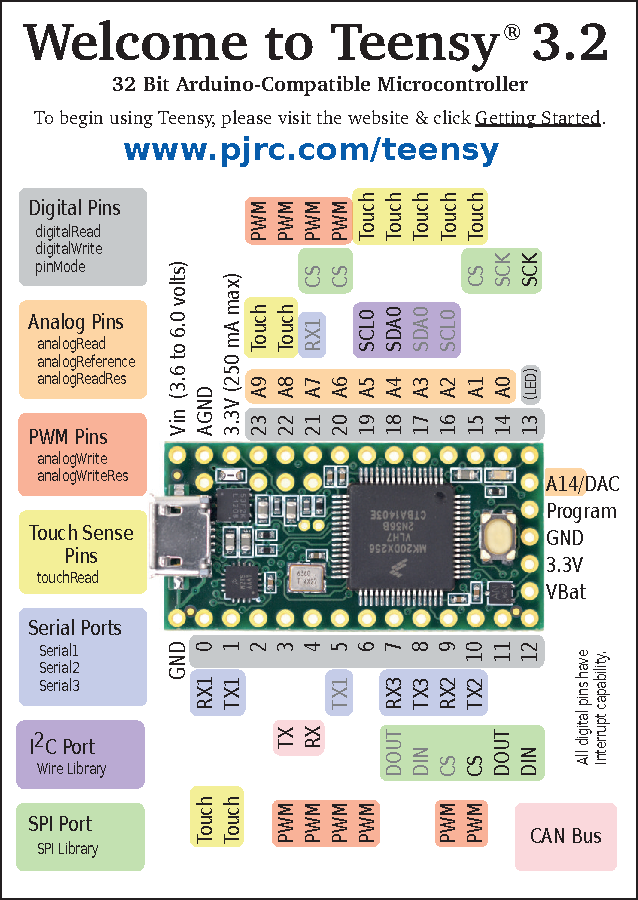
\includegraphics[width=6cm]{images/Teensy3.2 - 1.pdf}
    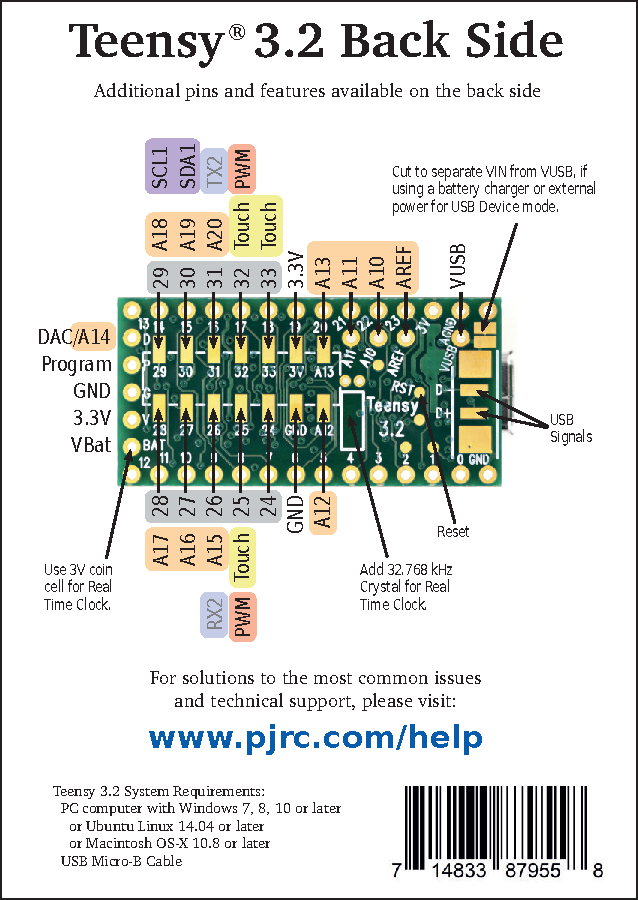
\includegraphics[width=6cm]{images/Teensy3.2 - 2.pdf}
    \caption{틴지 보드의 핀 맵(pin map)}
    \label{fig:enter-label}
\end{figure}


\begin{table}[H]
    \centering
    \caption{틴지 보드의 스펙}
    \begin{tabular}{l}
        \hline
        ARM Cortex-M4 at 72 MHz\\
        256K Flash, 64K RAM, 2K EEPROM\\
        USB device 12 Mbit/sec\\
        34 digital input/output pins, 12 PWM output pins\\
        21 analog input pins, 1 analog output pin, 12 capacitive sense pins\\
        3 serial, 1 SPI, 2 I2C ports\\
        1 I2S/TDM digital audio port\\
        1 CAN bus\\
        16 general purpose DMA channels\\
        RTC for date/time\\
        \hline
    \end{tabular}
    \label{Specification of Teensy Board}
\end{table}



\begin{figure}[H]
	\begin{center}
		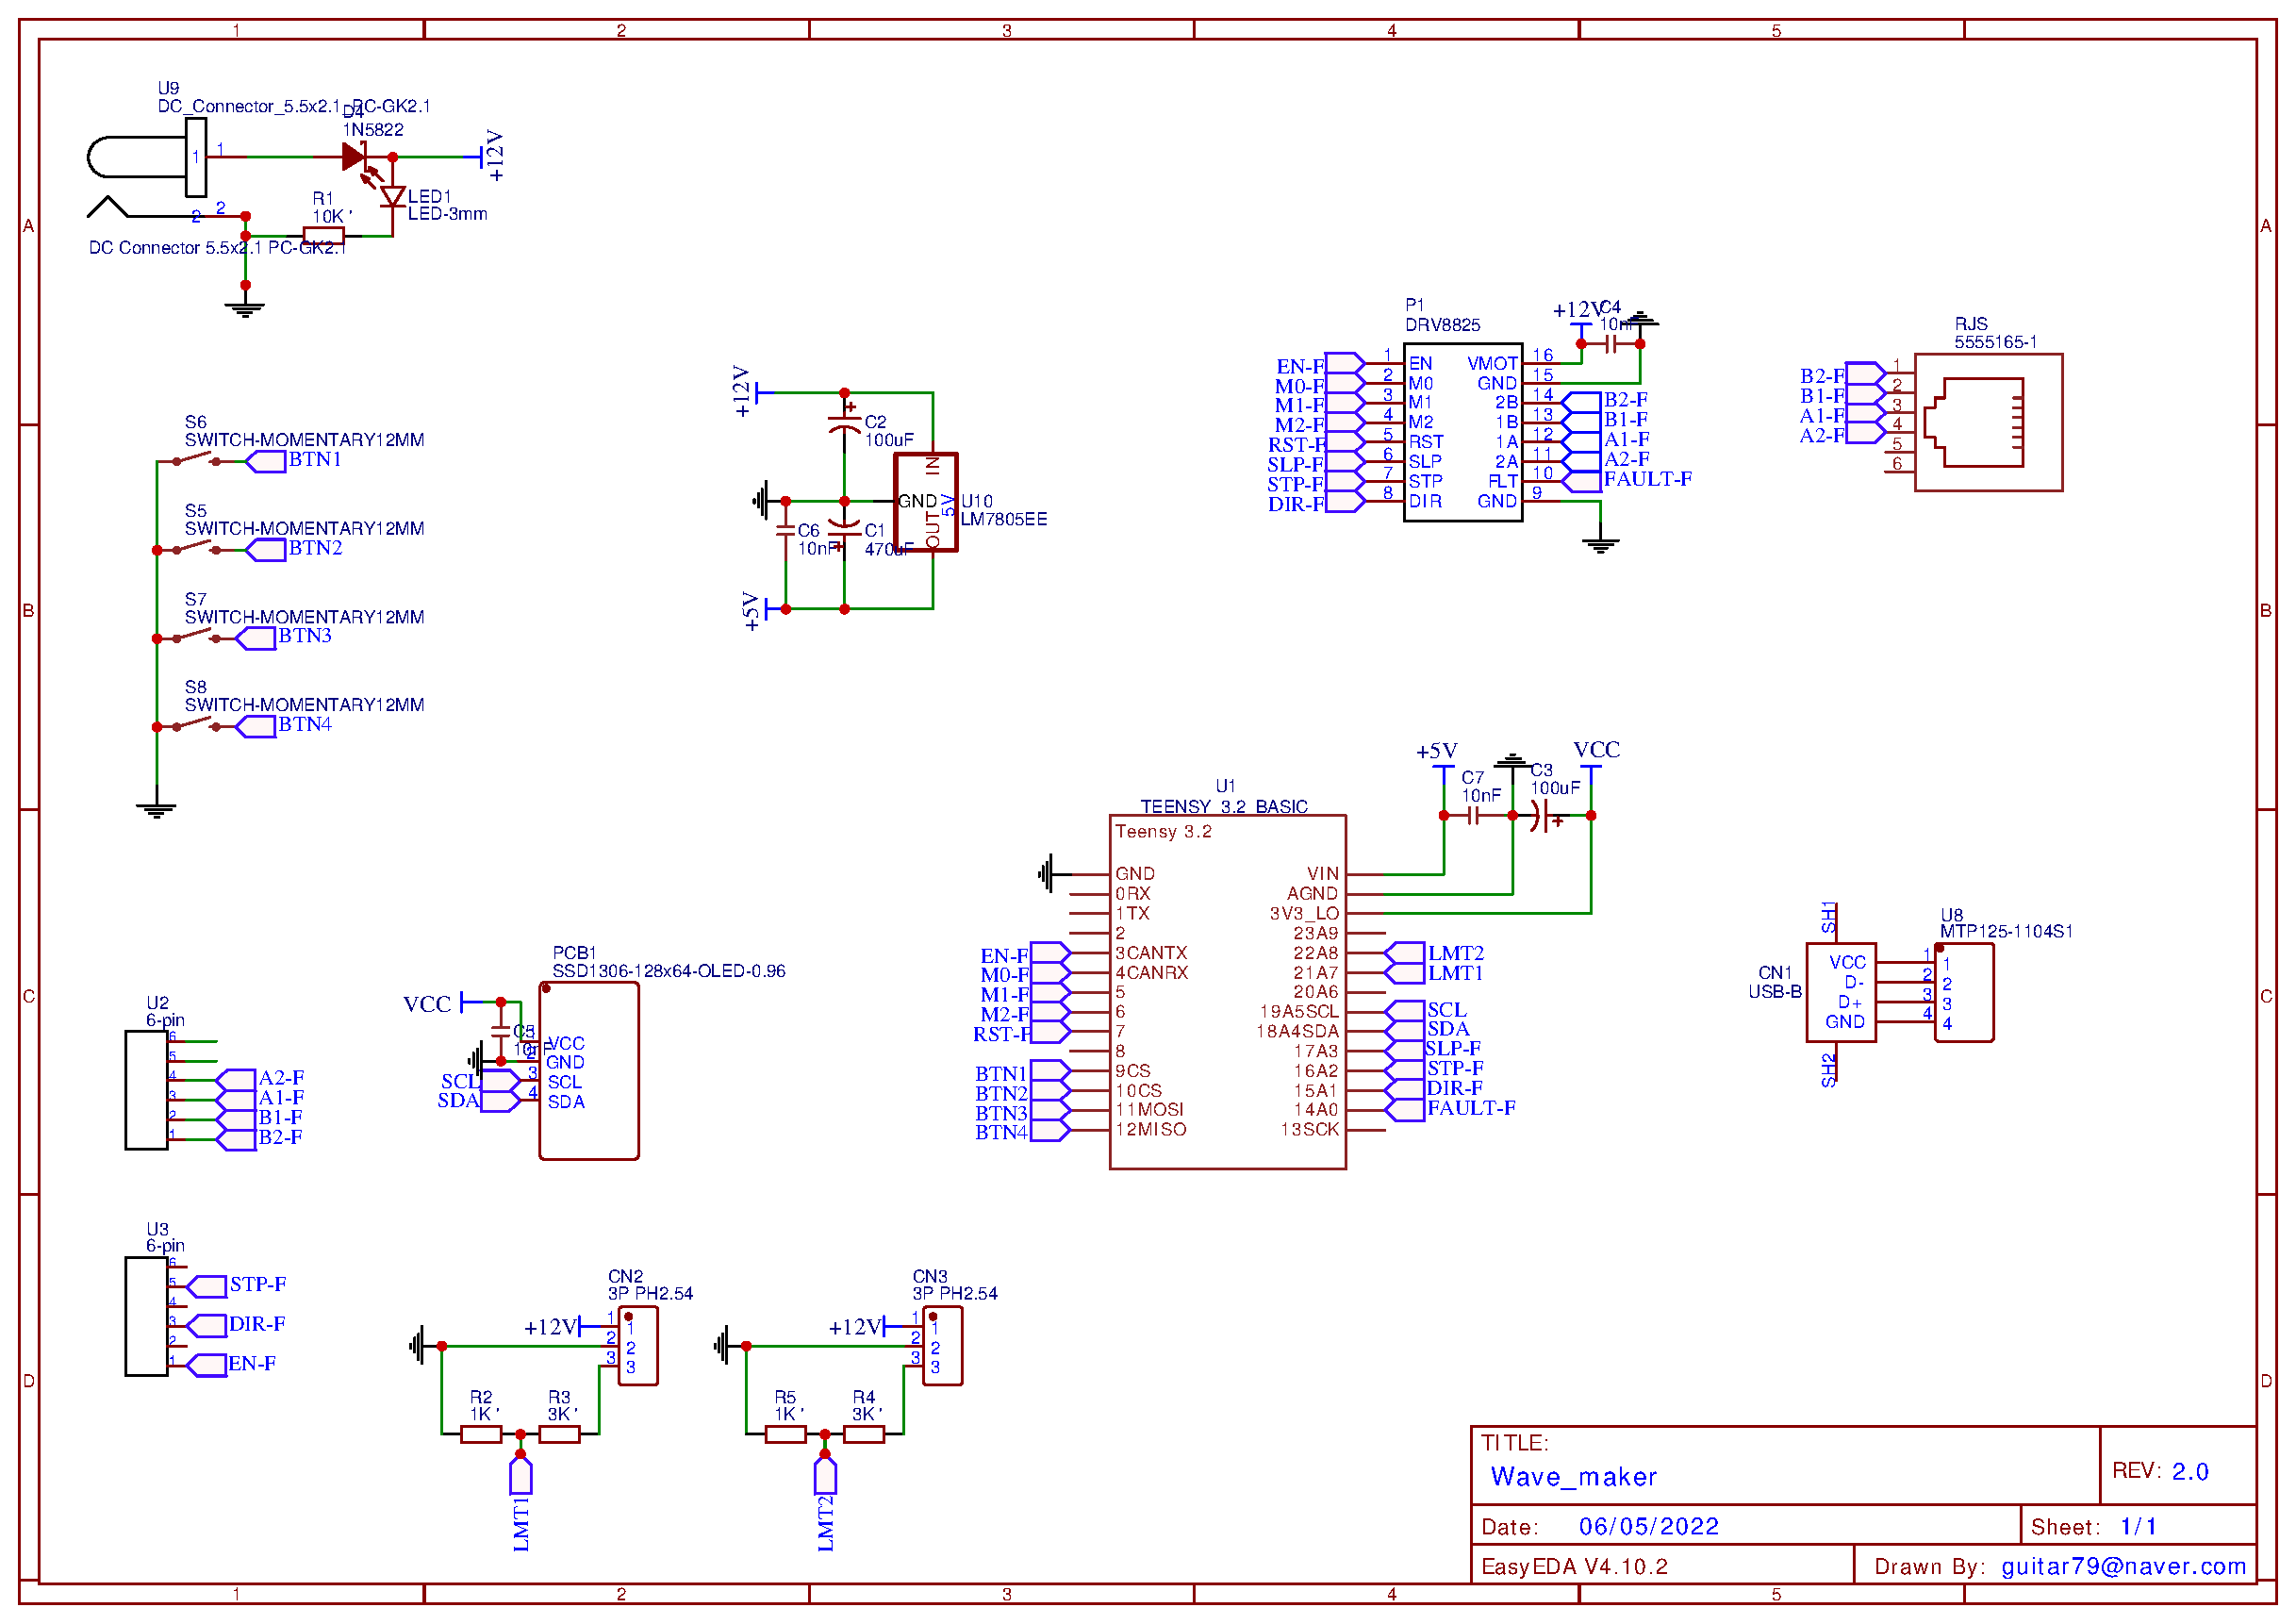
\includegraphics[height=5cm]{Schematic_Wave_maker_2-1_2022-11-24.pdf}
		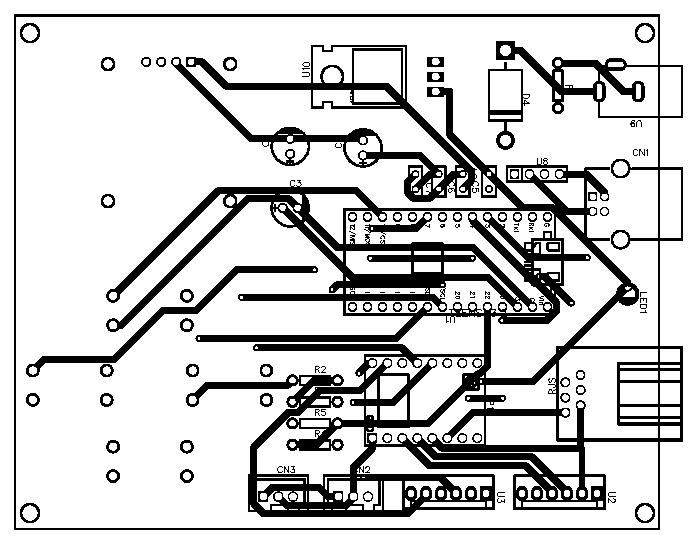
\includegraphics[height=5cm]{PCB_Wave_maker_2022-11-24.pdf}
        \caption{조파기 전자 회로 설계와 제작한 pcb}
		\label{PCB}
	\end{center}
\end{figure}


각 소자를 편리하게 다루기 위하여 pcb를 설계하였다. 틴지 보드 3.2는 3.2$\mathrm{V}$의 구동 전압이 필요하며 상세 스펙은 다음과 같다(표 \ref{Specification of Teensy Board}).



\begin{table}[H]
    \centering
    \caption{조파기 전자 회로에 사용된 부품}
    \label{Specification of Teensy Board}
\begin{tabular}{l|llll}
\hline
ID & Name                             & \multicolumn{2}{l}{Designator}  & Quantity \\ \hline
1  & 10nF                             & \multicolumn{2}{l}{C6,C4,C7,C5} & 4        \\
2  & 470uF                            & \multicolumn{2}{l}{C1}          & 1        \\
3  & 100uF                            & \multicolumn{2}{l}{C2,C3}       & 2        \\
4  & USB-B                            & \multicolumn{2}{l}{CN1}         & 1        \\
5  & 1N5822                           & \multicolumn{2}{l}{D4}          & 1        \\
6  & LED-3mm                          & \multicolumn{2}{l}{LED1}        & 1        \\
7  & DRV8825                          & \multicolumn{2}{l}{P1}          & 1        \\
8  & 10KΩ                             & \multicolumn{2}{l}{R1}          & 1        \\
9  & 5555165-1                        & \multicolumn{2}{l}{RJS}         & 1        \\
10 & TEENSY\_3.2\_BASIC               & \multicolumn{2}{l}{U1}          & 1        \\
11 & 6-pin                            & \multicolumn{2}{l}{U2}          & 1        \\
12 & MTP125-1104S1                    & \multicolumn{2}{l}{U8}          & 1        \\
13 & DC\_Connector\_5.5x2.1\_PC-GK2.1 & \multicolumn{2}{l}{U9}          & 1        \\
14 & LM7805EE                         & \multicolumn{2}{l}{U10}         & 1        \\
15 & SSD1306-128x64-OLED-0.96         & \multicolumn{2}{l}{PCB1}        & 1        \\
16 & Momentary Switch                 & \multicolumn{2}{l}{S1,S2,S3,S4} & 4       
\\ \hline
\end{tabular}
\end{table}


ST-M5045는 리니어 액츄에이터의 모터를 조절하는 모터 드라이버이며 옆의 스위치의 조작에 따라서 스텝 수와 전류 값을 조절하여 외부적으로도 모터 회전의 감도를 바꿀 수 있다.

\begin{table}[H]
    \centering
    \captionsetup{justification=centering}
    \caption{ST-M5045의 스펙}
    \begin{tabular}{ll}
        \hline
        \textbf{DC power input type $(\mathrm{V})$}  & \textbf{24$\sim$50}      \\
        \textbf{Output current $(\mathrm{A})$}       & \textbf{1$\sim$4.5}      \\
        \textbf{Mircostep}           & \textbf{2, 4, 8, 16, 32, 64, 128, 256, 5, 10, 25, 50, 125, 250               }                \\
        Protect form        & Overheated, Short-voltage, over-voltage, over-current protection \\
        Maximum pulse rate $(\mathrm{kHz})$ & 300             \\
        Dimensions               & $120\mathrm{~mm} \times92\mathrm{~mm}\times33\mathrm{~mm}$ \\
        % Weight                   & \textless{}280g \\
        Working environment & Temperature~~-$15\sim40\mathrm{\degree C}$, Humidity~\textless{}$90\%$ \\ 
        \hline
    \end{tabular}
    \label{Specification of ST-M5045}
\end{table}

여러 소자를 연결하여 구성한 조파기의 제어부는 그림 \ref{Wavemaker}\와 같다.

\begin{figure}[H]
	\begin{center}
		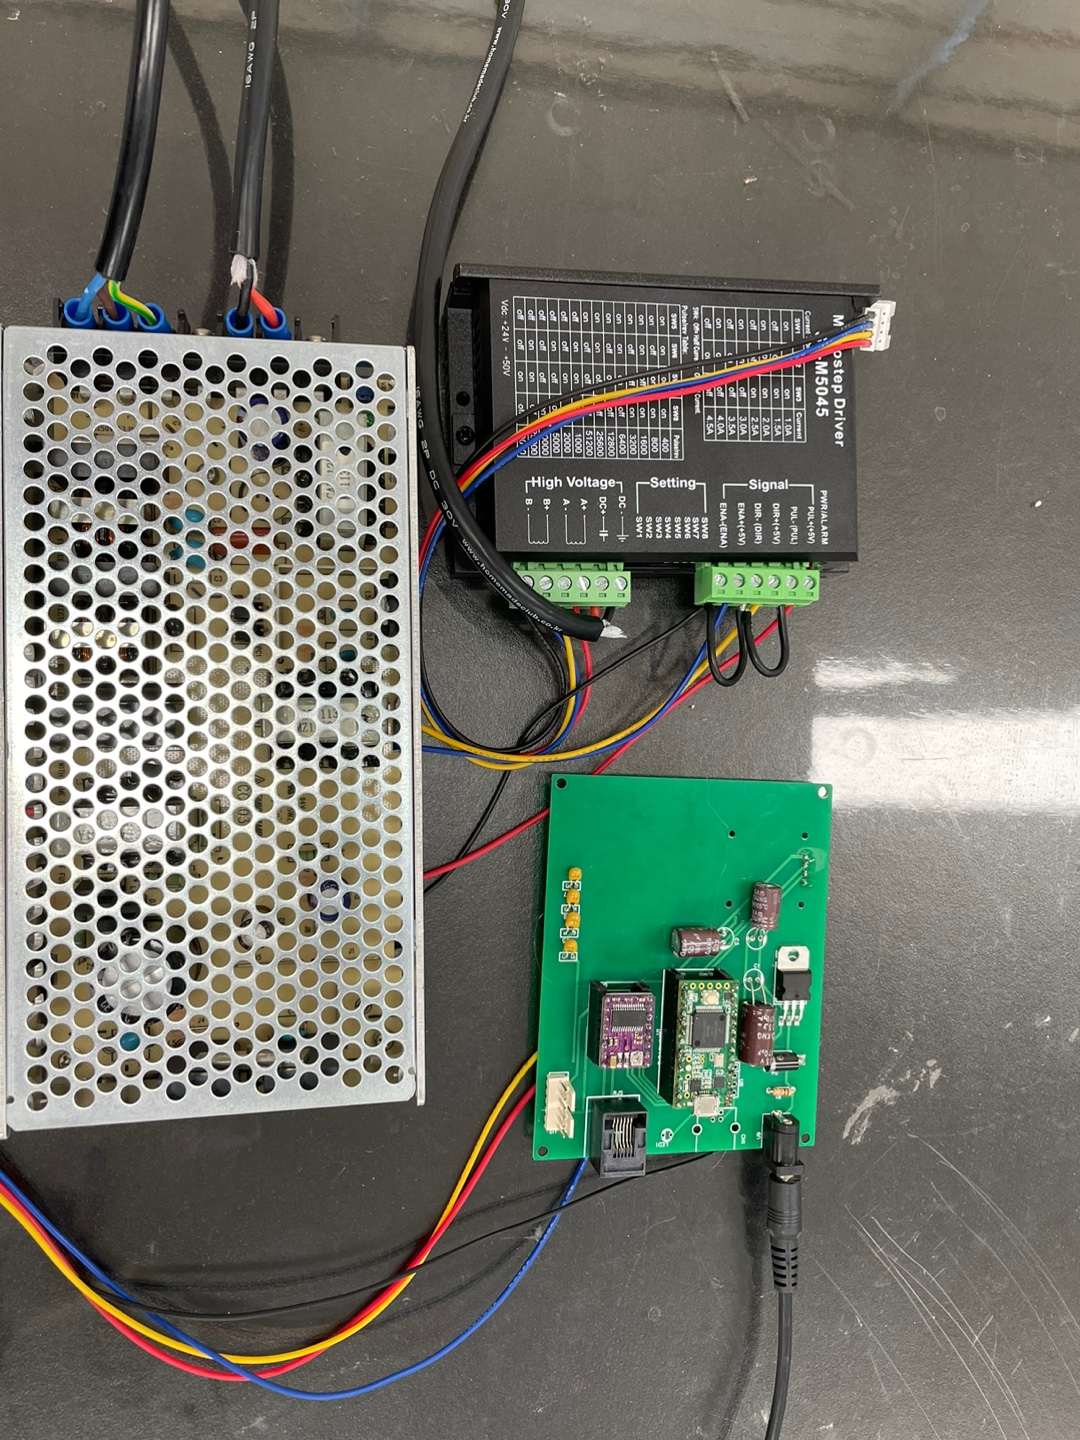
\includegraphics[clip, trim=0 100 100 100, angle=90, origin=c, width=.7\textwidth]{gdb}
		\caption{조파기 전자 회로와 모터 드라이버, 전원장치를 연결한 모습}
		\label{Wavemaker}
	\end{center}
\end{figure}


%Teensy Board 3.2, ST-M5045 스펙을 집어넣을 것.
%핀 연결은 Schematic이 있으니 굳이 따로 쓰지 말도록 하자.


% 하지만 파의 운동을 분석해보면 sin 파에 근접한 것이며 sin형으로 운동하도록 속도를 대입한 결과 판이 이상하게 운동하였다(그림 \ref{Motion of Motor}). 그리하여 제대로 sin형으로 운동할 수 있도록 다른 코드를 짰다. 조파기의 스텝 모터는 400 step 회전 시 $1~\rm{cm}$ 전진한다.

% \begin{figure}[H]
%     \centering
%     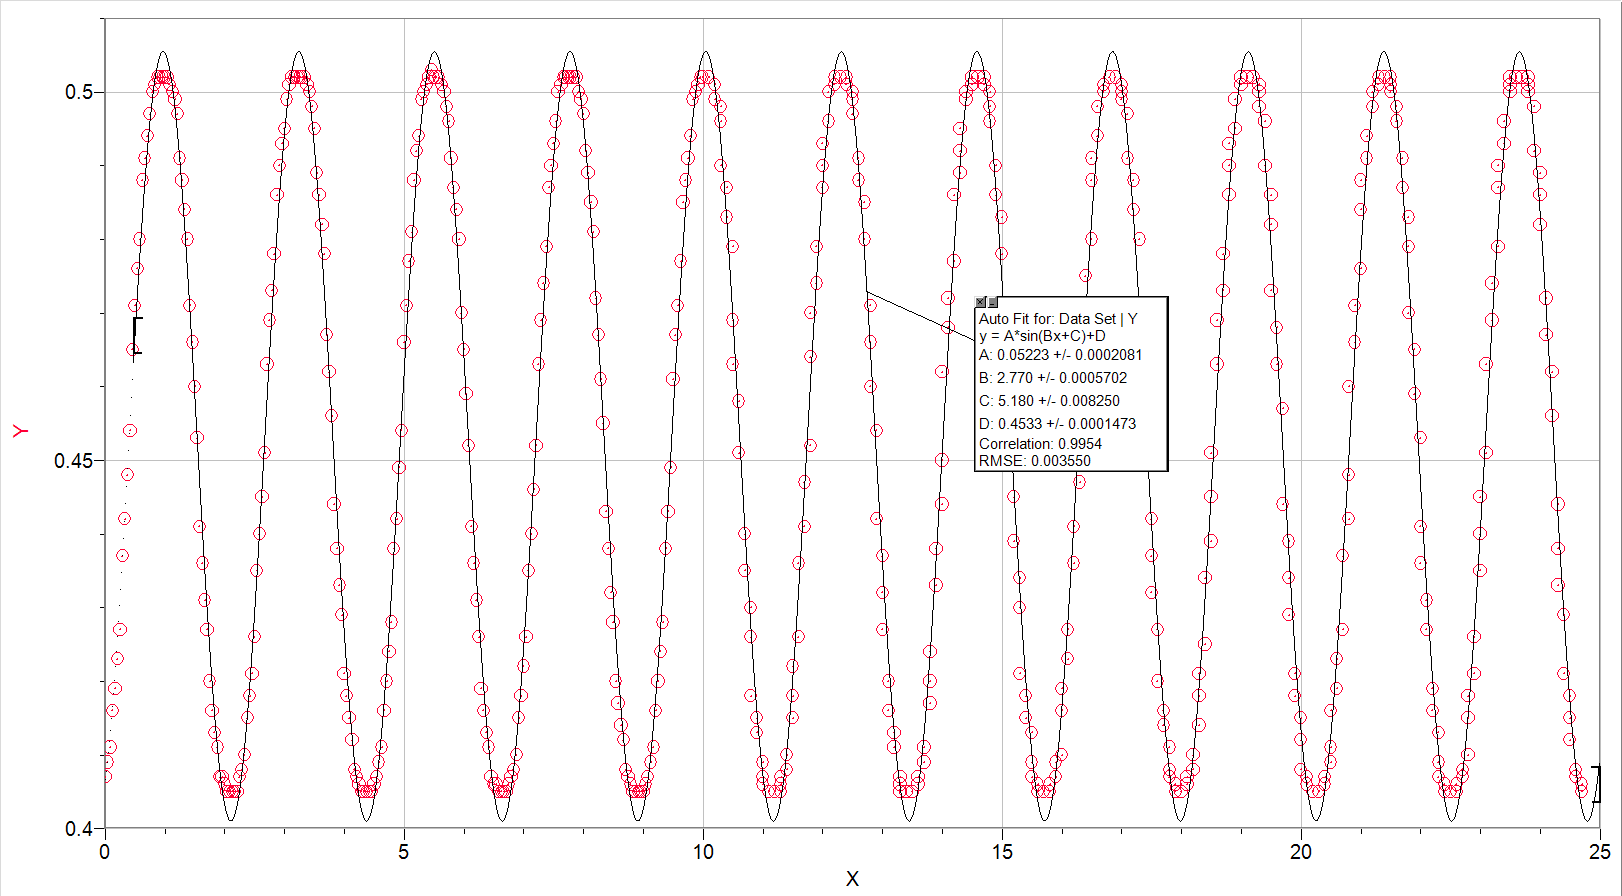
\includegraphics[height=4.5cm]{images/Linear_Motion.png}
%     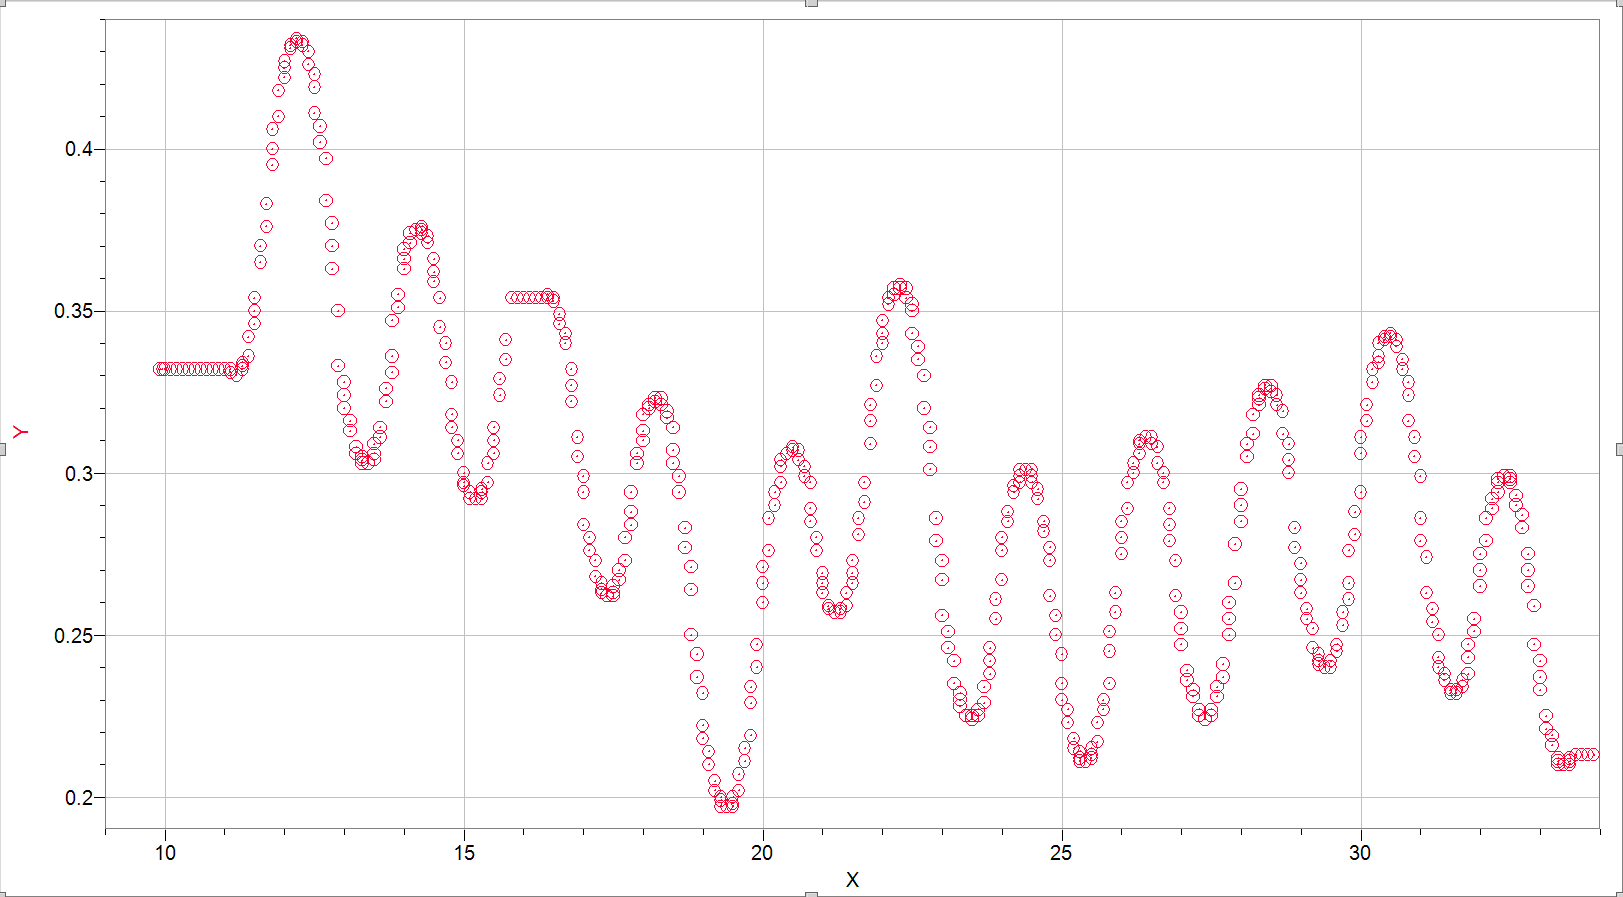
\includegraphics[height=4.5cm]{images/Sine_Motion.png}
%     \caption{모터의 선형 운동(좌)과 sin형 운동(우)}
%     \label{Motion of Motor}
% \end{figure}


\begin{figure}[H]
        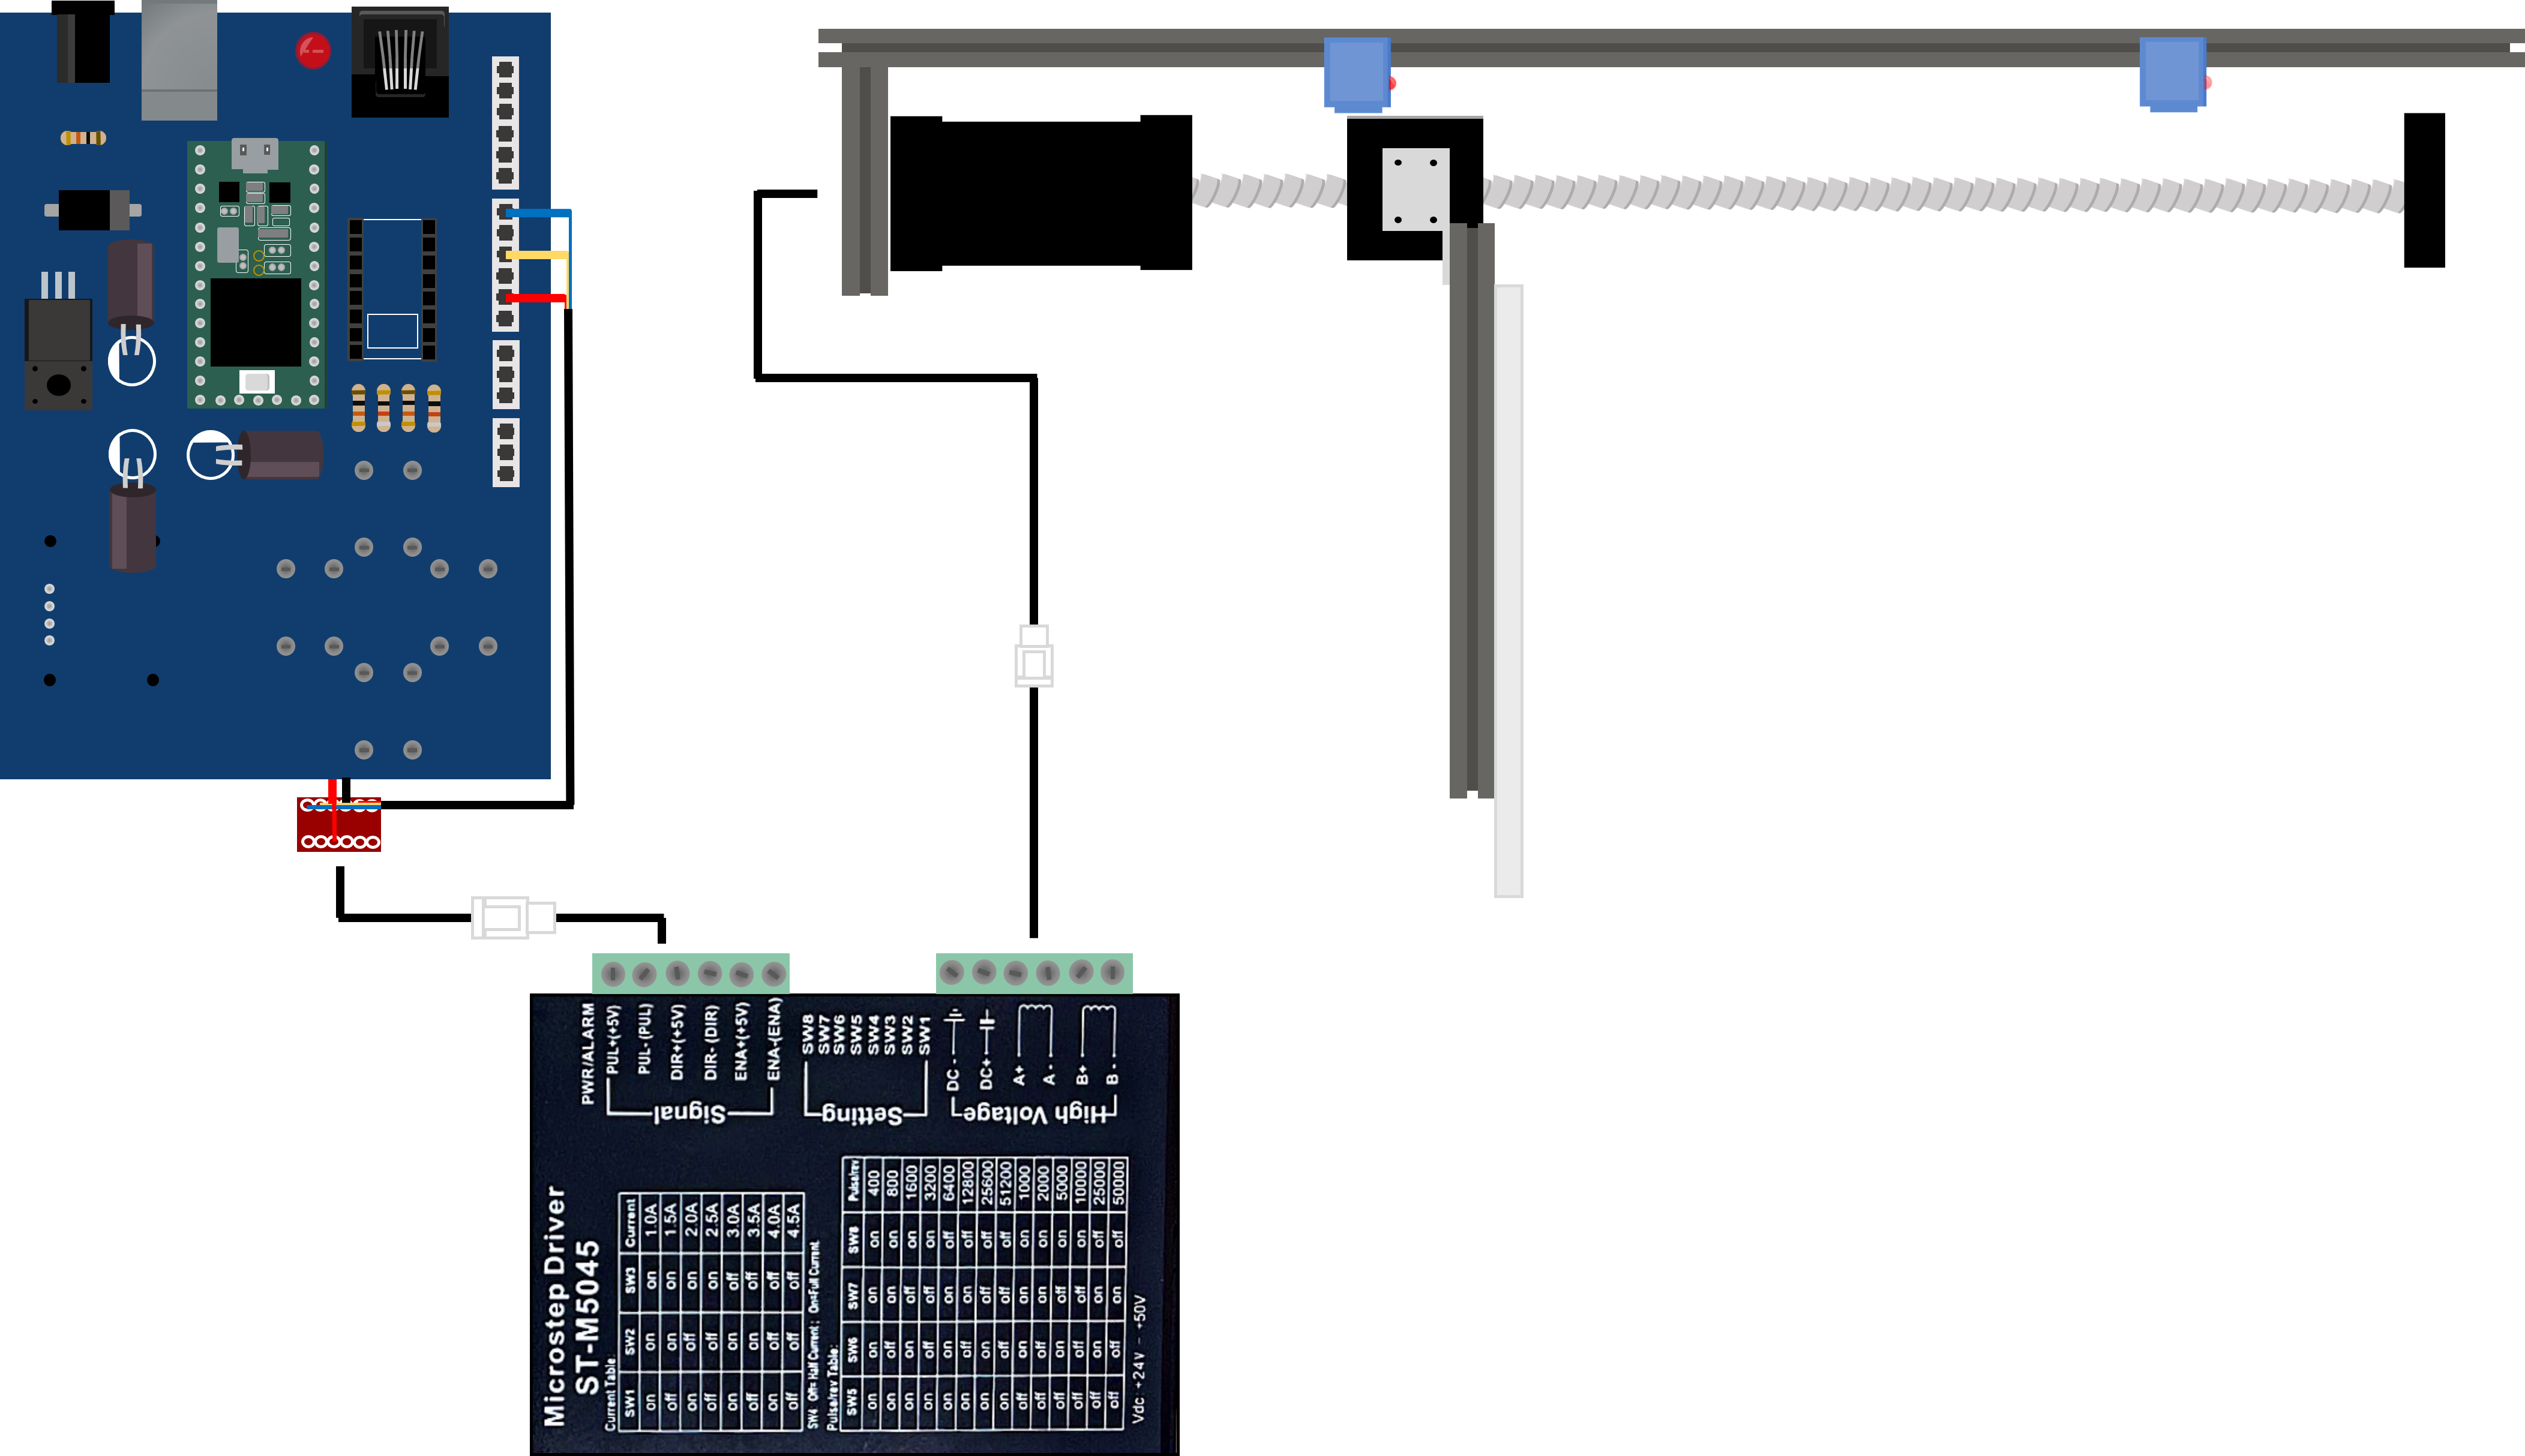
\includegraphics[width=0.9\textwidth]{images/wavemaker_control.png}
    \caption{조파기 전자 회로와 모터 드라이버, 전원장치를 연결한 모습}
    \label{wavemaker-structure}   
\end{figure}
%%%%%%%%%%%%%%%%%%%%%%%%%


\subsubsection{소프트웨어}
코딩은 Arduino를 틴지 보드에 적용할 수 있도록 컴파일러를 수정한 Teensyduino를 이용하였다. 기본적인 이동 코드는 전진, 후진이다. 스텝 모터 라이브러리는 AccelStepper, Stepper 등이 있으나 틴지 보드에서는 TeensyStep으로 모터를 더 빠르게 구동할 수 있었다. 버튼과 연계하여 각 버튼을 누를 때마다 왼쪽, 오른쪽으로 특정 변위만큼 이동하도록 할 수 있고 이를 반복하면 sin 파에 근접한 파를 만들 수 있다. 하지만 이는 근사적인 것이고 직접 변위를 대입하는 방식으로 코드를 짜서 조파기를 구동하였다.

\begin{figure}[H]
            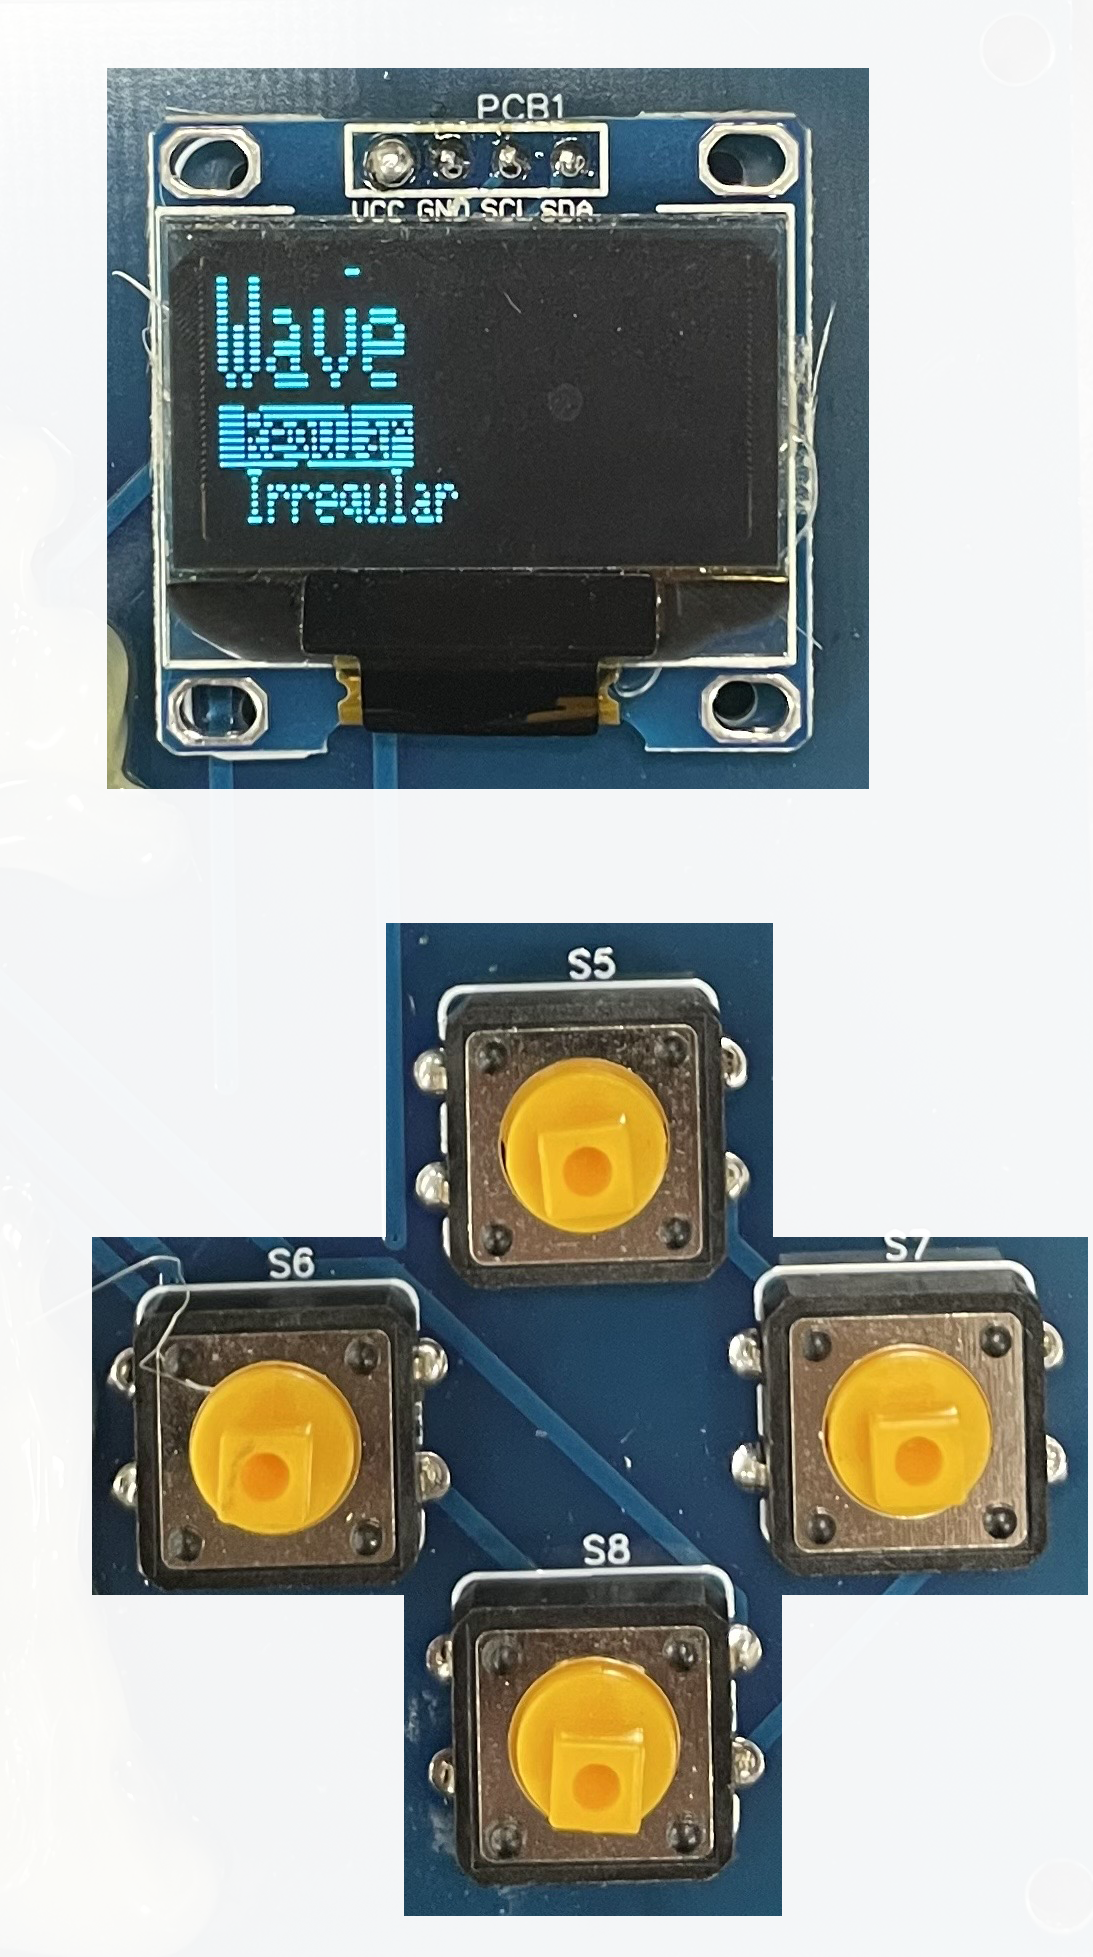
\includegraphics[trim=10 1050 100 0, clip, width=0.24\textwidth, height=3cm]{images/OLED1.png} 
            % (왼쪽, 아래(), 오른쪽, 위(숫자가 클수록 위에서 많이 잘림) )
            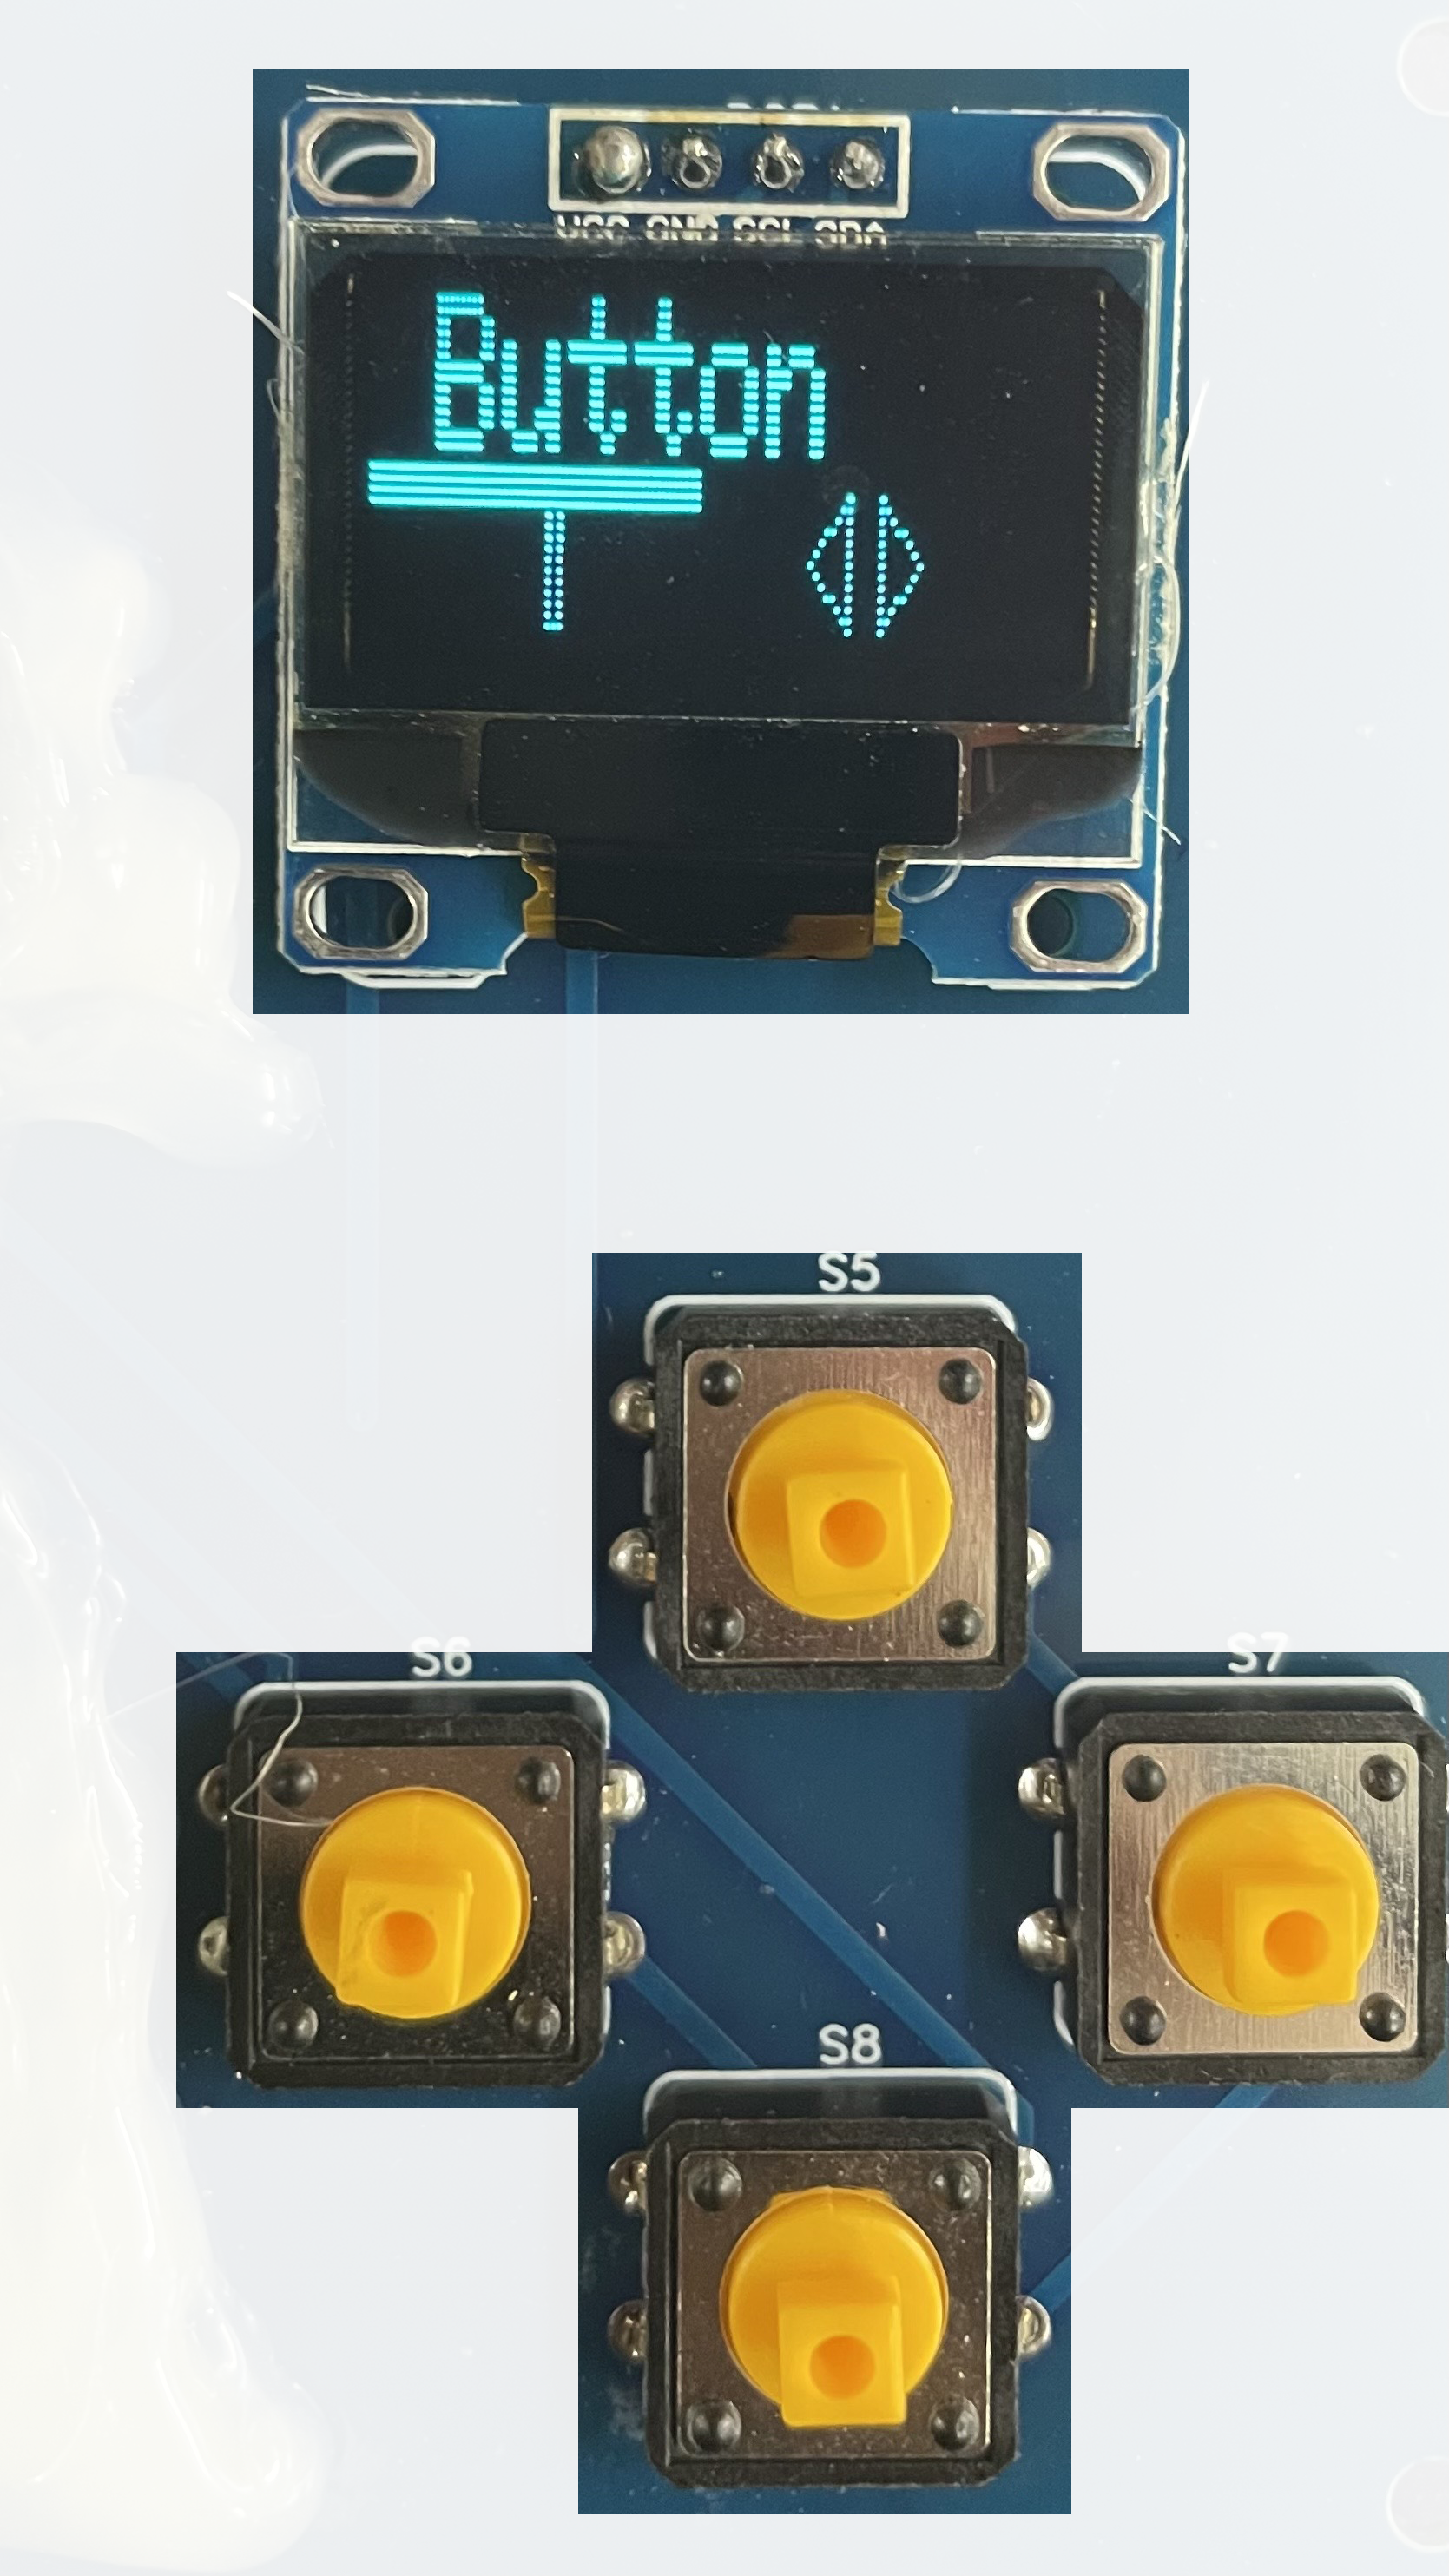
\includegraphics[trim=100 1550 100 0, clip, width=0.24\textwidth, height=3cm]{images/OLED2.png}
            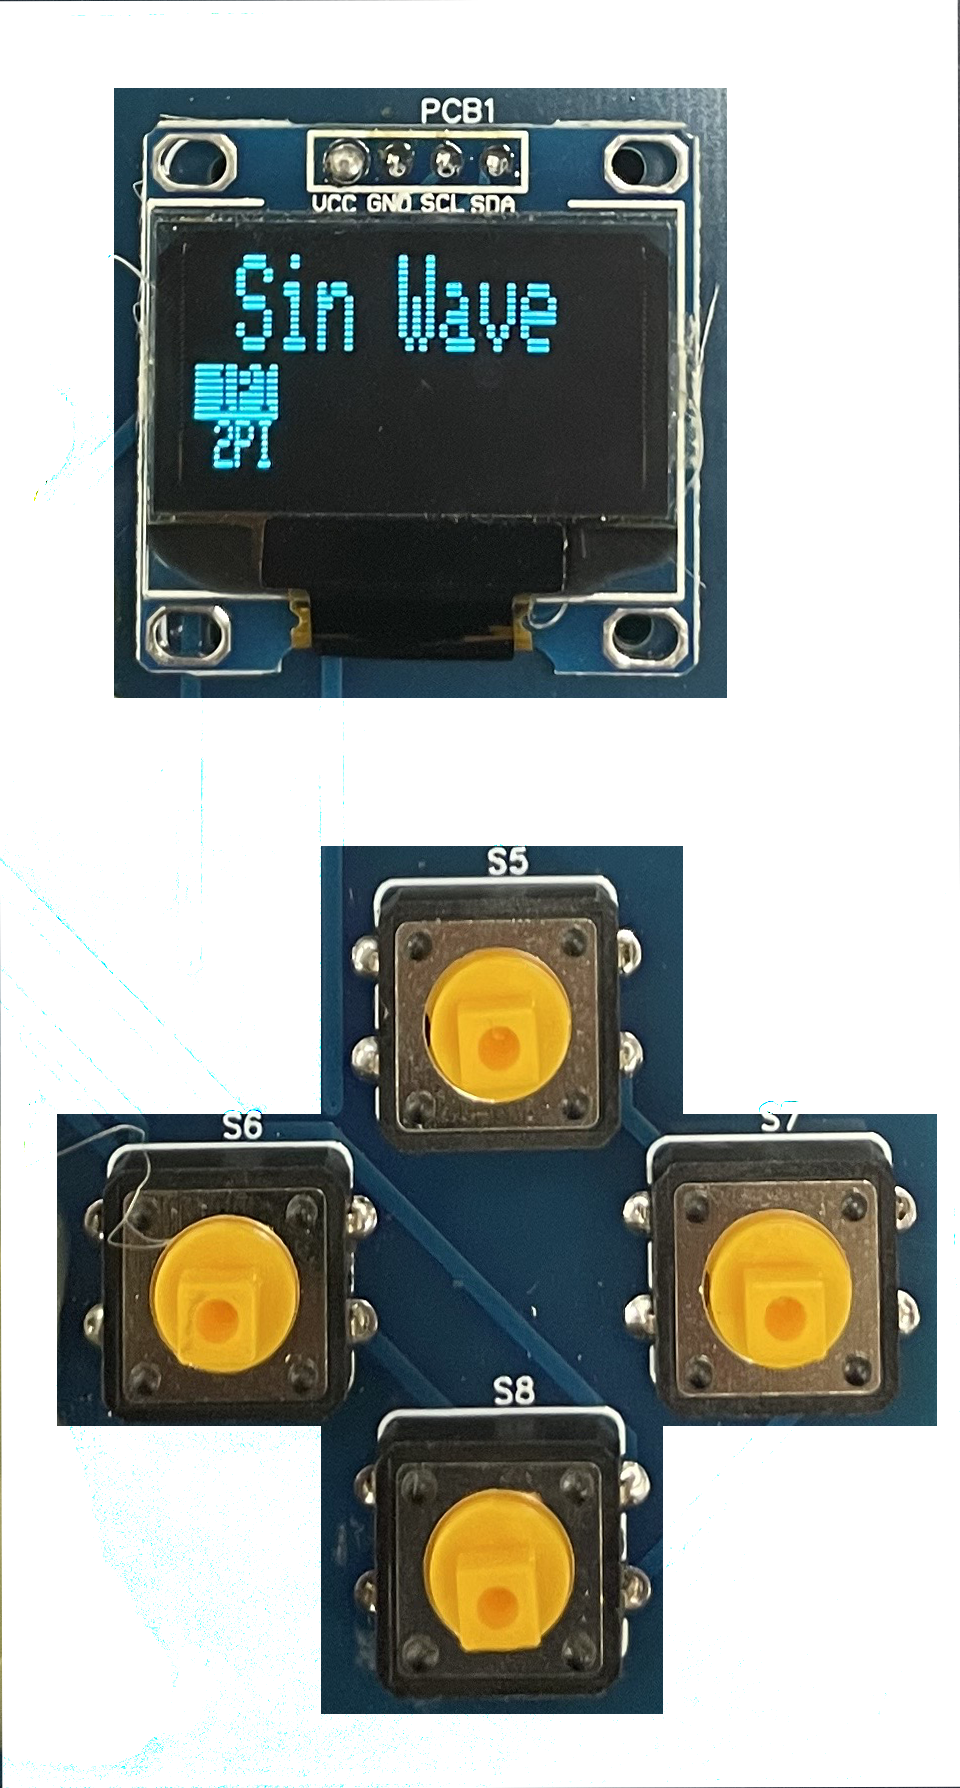
\includegraphics[trim=30 950 150 0,clip, width=0.24\textwidth, height=3cm]{images/OLED3.png}
            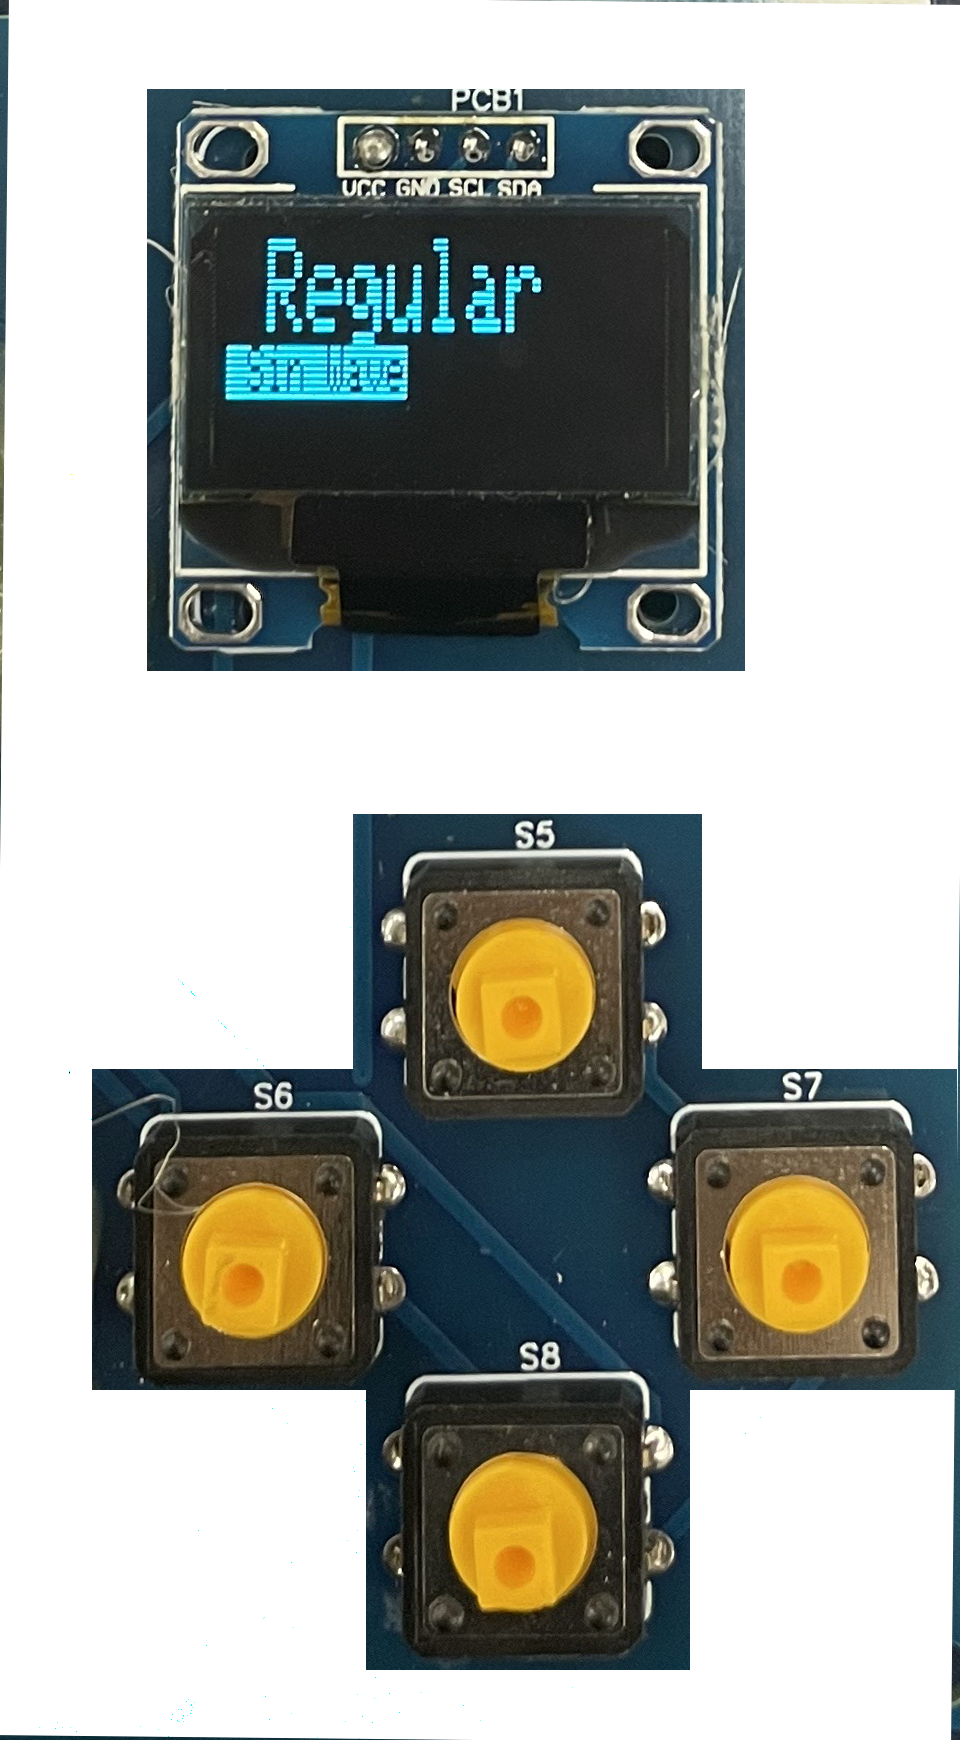
\includegraphics[trim=30 950 100 0, clip, width=0.24\textwidth, height=3cm]{images/OLED4.png}
        \caption{디스플레이 메뉴 동작 모습}
        \label{Oled}   
    \end{figure} 
    
전원을 켜면 Initialize가 실행된 후 메뉴 화면이 호출된다. 메뉴의 목록은 n진 트리의 형태로 구성되어 있으며, Wave 항목 아래에 Regular Wave, Irregular Wave, Button이 있고 각각을 버튼을 이용해 누르면 그 아래의 항목들이 호출되는 형태이다. Sin Wave의 항목에서는 변수 값을 선택해 원하는 값의 균형파를 생성할 수 있고, Button 항목에서는 원하는 방향으로 판을 움직일 수 있다. % 연구 과정
	\section{규칙파 검증 실험 및 결과}

\subsection{조파기 구동 코드}

\begin{algorithm}[h]
    \caption{Sinusoidal Motion}
    \label{Sinusoidal Motion}
    \begin{algorithmic}[1]
    \Procedure{Sinusoidal Motion}{$A, N, \Delta\phi$}\Comment{Move the motor by sinusoidal function}
        \For{$elapsed Time \geq 0$}
            \If{$elapsed Time \geq N$}
                \State {$elapsed Time$ = 0}
                \State {$target = f(n)$}%\Comment{In this case, $target$ = $A \sin${($n$ $\Delta$$\phi$)}}
                % \State {$target$ = $A \sin${($n$ $\Delta$$\phi$)}}
                \State {$n$ $\gets$ $n$ + 1}
                \State {Move $motor$ to $target$}
            \EndIf
        \EndFor
        \EndProcedure
    \end{algorithmic}
\end{algorithm}

조파기 구동 코드는 시간간격 $N$마다 ($N$은 $\mathrm{~ms}$ 단위이다) 각 변위를 $f(n)$으로 지정하는 방식으로 작동한다 (알고리즘 \ref{Sinusoidal Motion}). 이 함수가 $\sin$형이면 모터가 사인형 각 변위를 따라 움직일 것으로 기대할 수 있다. sin형 구동을 위한 코드의 $f(n)$은 다음과 같다.
\begin{equation}
    f(n) = A \sin(n \Delta\phi)
    \label{f(n)}
\end{equation}

하지만 실질적인 매개변수는 $A, \omega, N$이며 $A$는 진폭, $\omega$는 조파판 위상의 각진동수, $N$은 조파판의 변위를 업데이트하는 시간 간격이다. $\omega$는 다음과 같이 정의될 수 있다.

\begin{equation}
    \omega = \frac{\Delta\phi}{\Delta t} = \frac{\Delta\phi}{N}, ~\Delta\phi = N \omega
    \label{f(N)}
\end{equation}

즉, $N$과 $\omega$가 매개된 입력 신호의 식을 알 수 있다. $A$와 $\omega$는 코드에서의 입력값과 조파기 구동 시 판의 움직임에서 실제로 나타나는 값이 달라 그 관계를 파악하기 위한 실험이 필수적이며, $\omega$를 크게 할 경우 탈조가 날 수 있어 가능 범위를 파악해야 한다. $N$은 이론적으로 조파판의 움직임에 영향을 주는 요소가 아니어서 이를 고정하여 실험을 진행했으나, 판의 최대 변위와 최소 변위 지점에서 변위가 업데이트되어야 하므로 각진동수에 따른 $N$의 변화가 필요할 수 있다. 즉, 각진동수의 크기에 따라서 최선의 $N$이 있을 수 있다는 것이다.

\subsection{예비 실험}
$A$는 $5\mathrm{~cm}$, $N$은 50으로 고정한 후, $\omega$를 $0.4\pi$에서 $\pi$까지 $0.1\pi$ 간격으로 변화시키며 실험하고 추가로 $1.5\pi$에 대해 실험을 진행하였다. 
이 경우 판의 움직임을 분석했을 때 $\omega$가 증가함에 따라 진폭의 출력값이 감소하는 것을 확인할 수 있었다. 생성되는 파의 경우, sin파 형태와 유사하고 각진동수는 입력값과 동일했지만 진폭은 관계가 없어서 실험 구성 단계에서는 모터의 움직임만 분석하기로 결정하였다. 

\subsection{실험 구성}
생성파의 분석이 필요치 않으므로 조파기의 모터 대신 작은 모터에 회로를 연결하여 모터의 움직임이 sin 형태인지를 확인하였다. 이는 시리얼 모니터에 현재 각 위치를 출력하여 알 수 있다. 각진동수의 출력값은 입력값과 일치하나 진폭은 달랐으며, $\omega$가 클수록 진폭의 출력값이 감소하였다 (그림 \ref{PreExperiment}).

\begin{figure}[H]
    \centering
    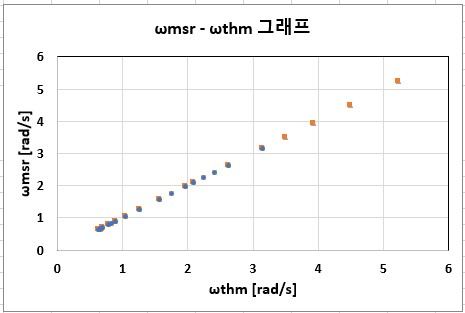
\includegraphics[height=5cm]{images/PreExperiment_Graph(Omega-Omega)-junlam.jpg}
    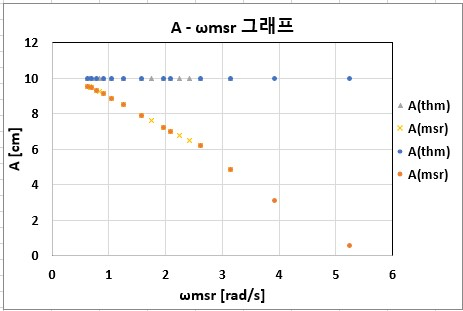
\includegraphics[height=5cm]{images/PreExperiment_Graph(A-Omega)-junlam.jpg}
    \caption{$\omega_{msr}$(측정값)에 대한 $\omega_{thm}$(입력값) (좌),  $\omega_{msr}$에 대한 진폭 $A_{msr}$(측정값) (우) - 예비 실험}
    \label{PreExperiment}
\end{figure}

그러므로 우리가 파를 생성하려고 할 때 구동 코드의 매개변수에 따른 판의 움직임과 생성되는 파 2개를 관찰해야 한다. 그리고 두 파의 진폭과 각진동수를 코드의 값과 비교하여 관계를 파악하는 것을 목표로 한다.

\begin{figure}[H]
    \centering
    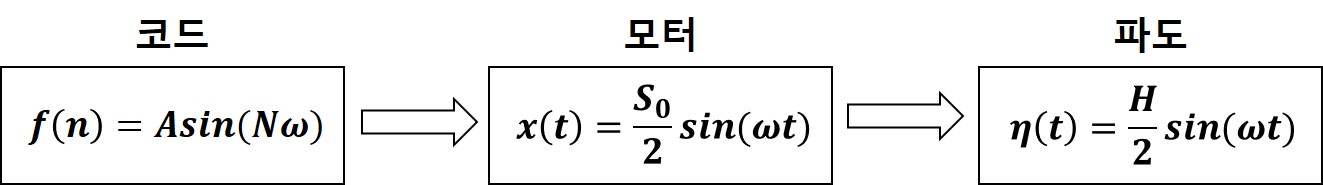
\includegraphics[width=12cm]{images/Flow_Chart(Analysis System_Kor).jpg}
    \caption{조파기 검증 실험의 흐름도}
    \label{Flow_Chart}
\end{figure}

비록 $S_0$와 $A$의 관계는 알 수 없으나 $S_0$와 $H$의 관계는 이론적 배경의 식을 따를 것으로 기대할 수 있으며 파가 sin형이 아니더라도 FFT 분석을 통해서 $\omega$를 구할 경우 세 파동에서 일관될 것이라고 예측할 수 있다.
이를 제대로 검증하기 위해서는 다양한 조건에 대한 데이터가 필요하며 이론적 분석과 예비 실험을 통해 정한 범위는 $A$는 $1\mathrm{~cm}$부터 $10\mathrm{~cm}$까지 $1\mathrm{~cm}$ 간격으로, $\omega$는 $3$부터 $12$까지 $1$ 간격으로 변화시키는 것이다. $N$은 50으로 고정시켰다 (단, 수심은 $15\mathrm{cm}$로 고정하였다).

%실험한 내용을 집어넣어야 함.

%실험계의 모식도가 필요함. 혹은 사진이라도.
\subsection{성능 검증 실험 결과}

\begin{figure}[H]
    \centering
    \begin{tabular}{ll}
        \begin{filecontents*}{A.dat}
w_msr	A_thm	A_msr
0.6272	10	9.515
0.6275	10	9.532
0.6541	10	9.523
0.6681	10	9.499
0.6826	10	9.48
0.6978	10	9.456
0.6978	10	9.449
0.7849	10	9.326
0.785	10	9.318
0.8263	10	9.26
0.8971	10	9.138
0.8971	10	9.137
1.047	10	8.883
1.047	10	8.876
1.256	10	8.498
1.256	10	8.492
1.57	10	7.916
1.57	10	7.903
1.744	10	7.588
1.962	10	7.206
1.962	10	7.197
2.093	10	6.988
2.093	10	6.978
2.243	10	6.749
2.415	10	6.489
2.617	10	6.218
2.618   10	6.214
3.141	10	4.837
3.141	10	4.837
3.927	10	3.093
5.236	10	0.5795
        \end{filecontents*}

        \begin{tikzpicture}[
                %Environment Cfg.
                %font=\bfseries\sffamily,
            ]
            \begin{axis}[
                width=6cm,
                height=6cm,
                at={(0,0)},
                ymin=0,
                ymax=13,
                xmin=0,
                xmax=6,
                grid=both,
                minor tick num =5,
                minor tick style={draw=none},
                minor grid style={thin,color=black!10},
                major grid style={thin,color=black!10},
                %ylabel style={rotate=90},
                ylabel={$A_{plate}~\left[\mathrm{~cm}\right]$},
                xlabel={$\omega_{msr}~\left[\mathrm{~rad/s}\right]$},
                tick align=outside,
                axis x line*=middle,
                axis y line*=none,
                xtick={0,2,...,16},
                ytick={0,2,...,16},
                %xlabel style={color=blue!50!cyan},
                %ylabel style={align=center,rotate=-90,color=blue!50!cyan},
                x tick label style={
                    /pgf/number format/assume math mode, font=\sf\scriptsize},
                y tick label style={
                    /pgf/number format/assume math mode, font=\sf\scriptsize},
                legend cell align = {left},
                legend pos = north west,
                legend style={nodes={scale=0.5, transform shape}},
                ]
                \addplot [%only marks, 
                    mark size=1pt,
                    mark=o, 
                    %mark options={solid}, 
                    %smooth,
                    ] 
                table [x=w_msr, y=A_thm] {A.dat};
                \addlegendentry{$A_{thm} - \omega_{msr}$}
                \addplot [%only marks, 
                    mark = +,
                    mark size=1pt,
                    ]
                table [x=w_msr, y=A_msr] {A.dat};
                \addlegendentry{$A_{msr} - \omega_{msr}$}
            \end{axis}
        \end{tikzpicture}
        
        &
        
        \begin{filecontents}{B.dat}
                    wthm   wPlate
0.6283	0.6272
0.6981	0.6978
0.7854	0.785
0.8976	0.8971
1.0472	1.047
1.2566	1.256
1.5708	1.57
1.9635	1.962
2.0944	2.093
2.6180	2.617
3.1416	3.141
3.9270	3.918
5.2360	5.236
4.4880	4.487
3.9270	3.919
3.4907	3.49
0.6283	0.6275
0.6545	0.6541
0.6684	0.6681
0.6830	0.6826
0.6981	0.6978
0.7854	0.7849
0.8267	0.8263
0.8976	0.8971
1.0472	1.047
1.2566	1.256
1.5708	1.57
1.7453	1.744
1.9635	1.962
2.0944	2.093
2.2440	2.243
2.4166	2.415
2.6180	2.617
3.1416	3.141
            \end{filecontents}
        
            \begin{tikzpicture}[
                    %Environment Cfg.
                    font=\bfseries\sffamily,
                ]
                    \begin{axis}[
                        width=6cm,
                        height=6cm,
                        at={(0,0)},
                        ymin=0,
                        ymax=6,
                        xmin=0,
                        xmax=6,
                        grid=both,
                        minor tick num =5,
                        minor tick style={draw=none},
                        minor grid style={thin,color=black!10},
                        major grid style={thin,color=black!10},
                        %ylabel style={rotate=90},
                        ylabel={$\omega_{msr}~\left[\mathrm{rad/s}\right]$},
                        xlabel={$\omega_{thm}~\left[\mathrm{rad/s}\right]$},
                        tick align=outside,
                        axis x line*=middle,
                        axis y line*=none,
                        xtick={0,2,...,16},
                        ytick={0,2,...,16},
                        %xlabel style={color=blue!50!cyan},
                        %ylabel style={align=center,rotate=-90,color=blue!50!cyan},
                        x tick label style={
                            /pgf/number format/assume math mode, font=\sf\scriptsize},
                        y tick label style={
                        /pgf/number format/assume math mode, font=\sf\scriptsize},
                        legend cell align = {left},
                        legend pos = north west,
                        legend style={nodes={scale=0.5, transform shape}},
                        ]
                        \addplot [only marks, 
                            mark size=1pt,
                            mark=o, 
                            ]
                            table [x=wthm, y=wPlate] {B.dat};
                           \addlegendentry{$ \omega_{msr} - \omega_{thm}$}
                    \end{axis}
        \end{tikzpicture}
    \end{tabular}
    
    \begin{tikzpicture} [remember picture, overlay]
        \node at (-5.8, 0.6) {\scriptsize{(a)}};
        \node at (2.0, 0.6) {\scriptsize{(b)}};
    \end{tikzpicture}
    \caption{$\omega_{msr} - \omega_{thm}$ graph - (a) wave (b) plate}
    \label{PreExperiment}
\end{figure}





\begin{figure}[H]
    \centering
    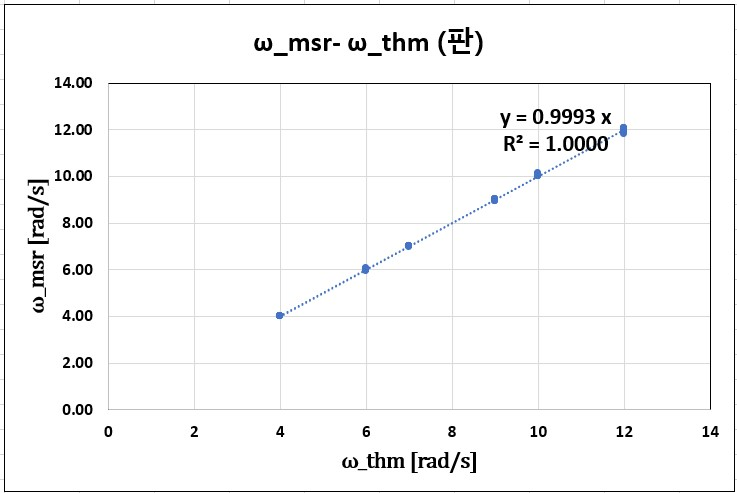
\includegraphics[height=5cm]{images/Experiment(omega_thm-omega_msr)_Plate_Kor.jpg}
    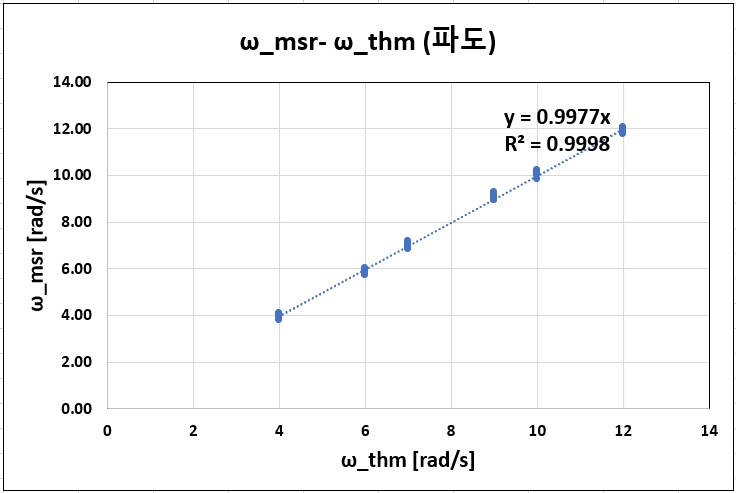
\includegraphics[height=5cm]{images/Experiment(omega_thm-omega_msr)_Wave_Kor.jpg}
    \caption{측정한 $\omega_{msr}$에 대한 코드의 $\omega_{thm}$ (좌),  $\omega_{msr}$에 대한 측정 진폭 $A_{msr}$ (우) - 검증 실험}
    \label{ExperimentGraph - 1, 2}
\end{figure}

그림 \ref{ExperimentGraph - 1, 2}에서 알 수 있듯이 $\omega$는 코드에서 대입한 값과 판, 파도 모두 같은 값을 띔을 알 수 있다 (두 그래프 모두 선형 관계를 만족하며($R^2 > 0.99$) 그 기울기는 약 1.000이다). 또, 분산 관계식과 식 \ref{eq:5}을 통해 주어진 $\omega$에 대한 $H/S$를 예측할 수 있고 이를 측정값과 비교해보았다 (그림 \ref{H/S Graph}).

\begin{figure}[H]
    \centering
    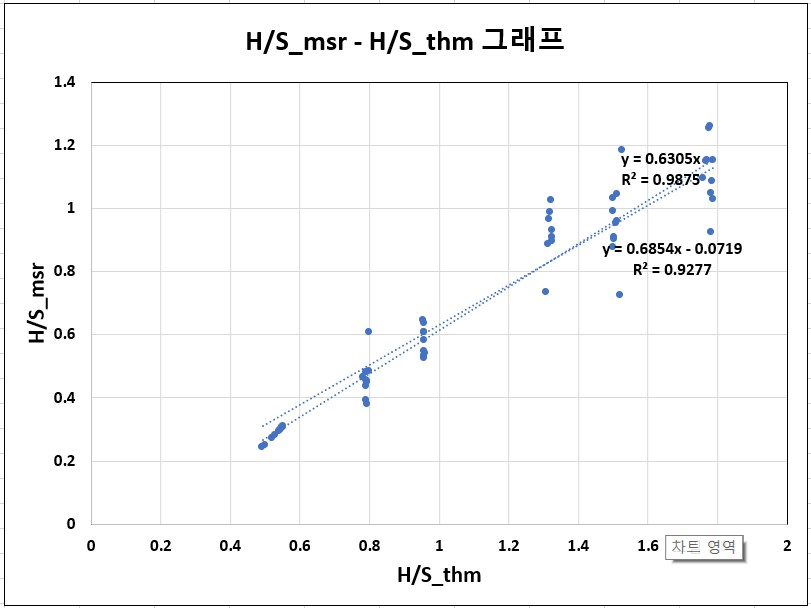
\includegraphics[width=0.70\textwidth]{images/Experiment(H.S_thm-H.S_msr).jpg}
    \caption{$H/S_{msr} - H/S_{thm}$ 그래프}
    \label{H/S Graph}
\end{figure}

$H/S$는 선형 관계를 만족한다고 볼 수 있다. 측정값이 구간으로 나타났으나 이는 불확도 내의 값으로 취급할 수 있으며 선형 추세선의 기울기가 $1.000$은 아니지만 선형 추세를 통해 매개변수로부터 $H/S$를 예측할 수 있다.

\begin{figure}[H]
    \centering
    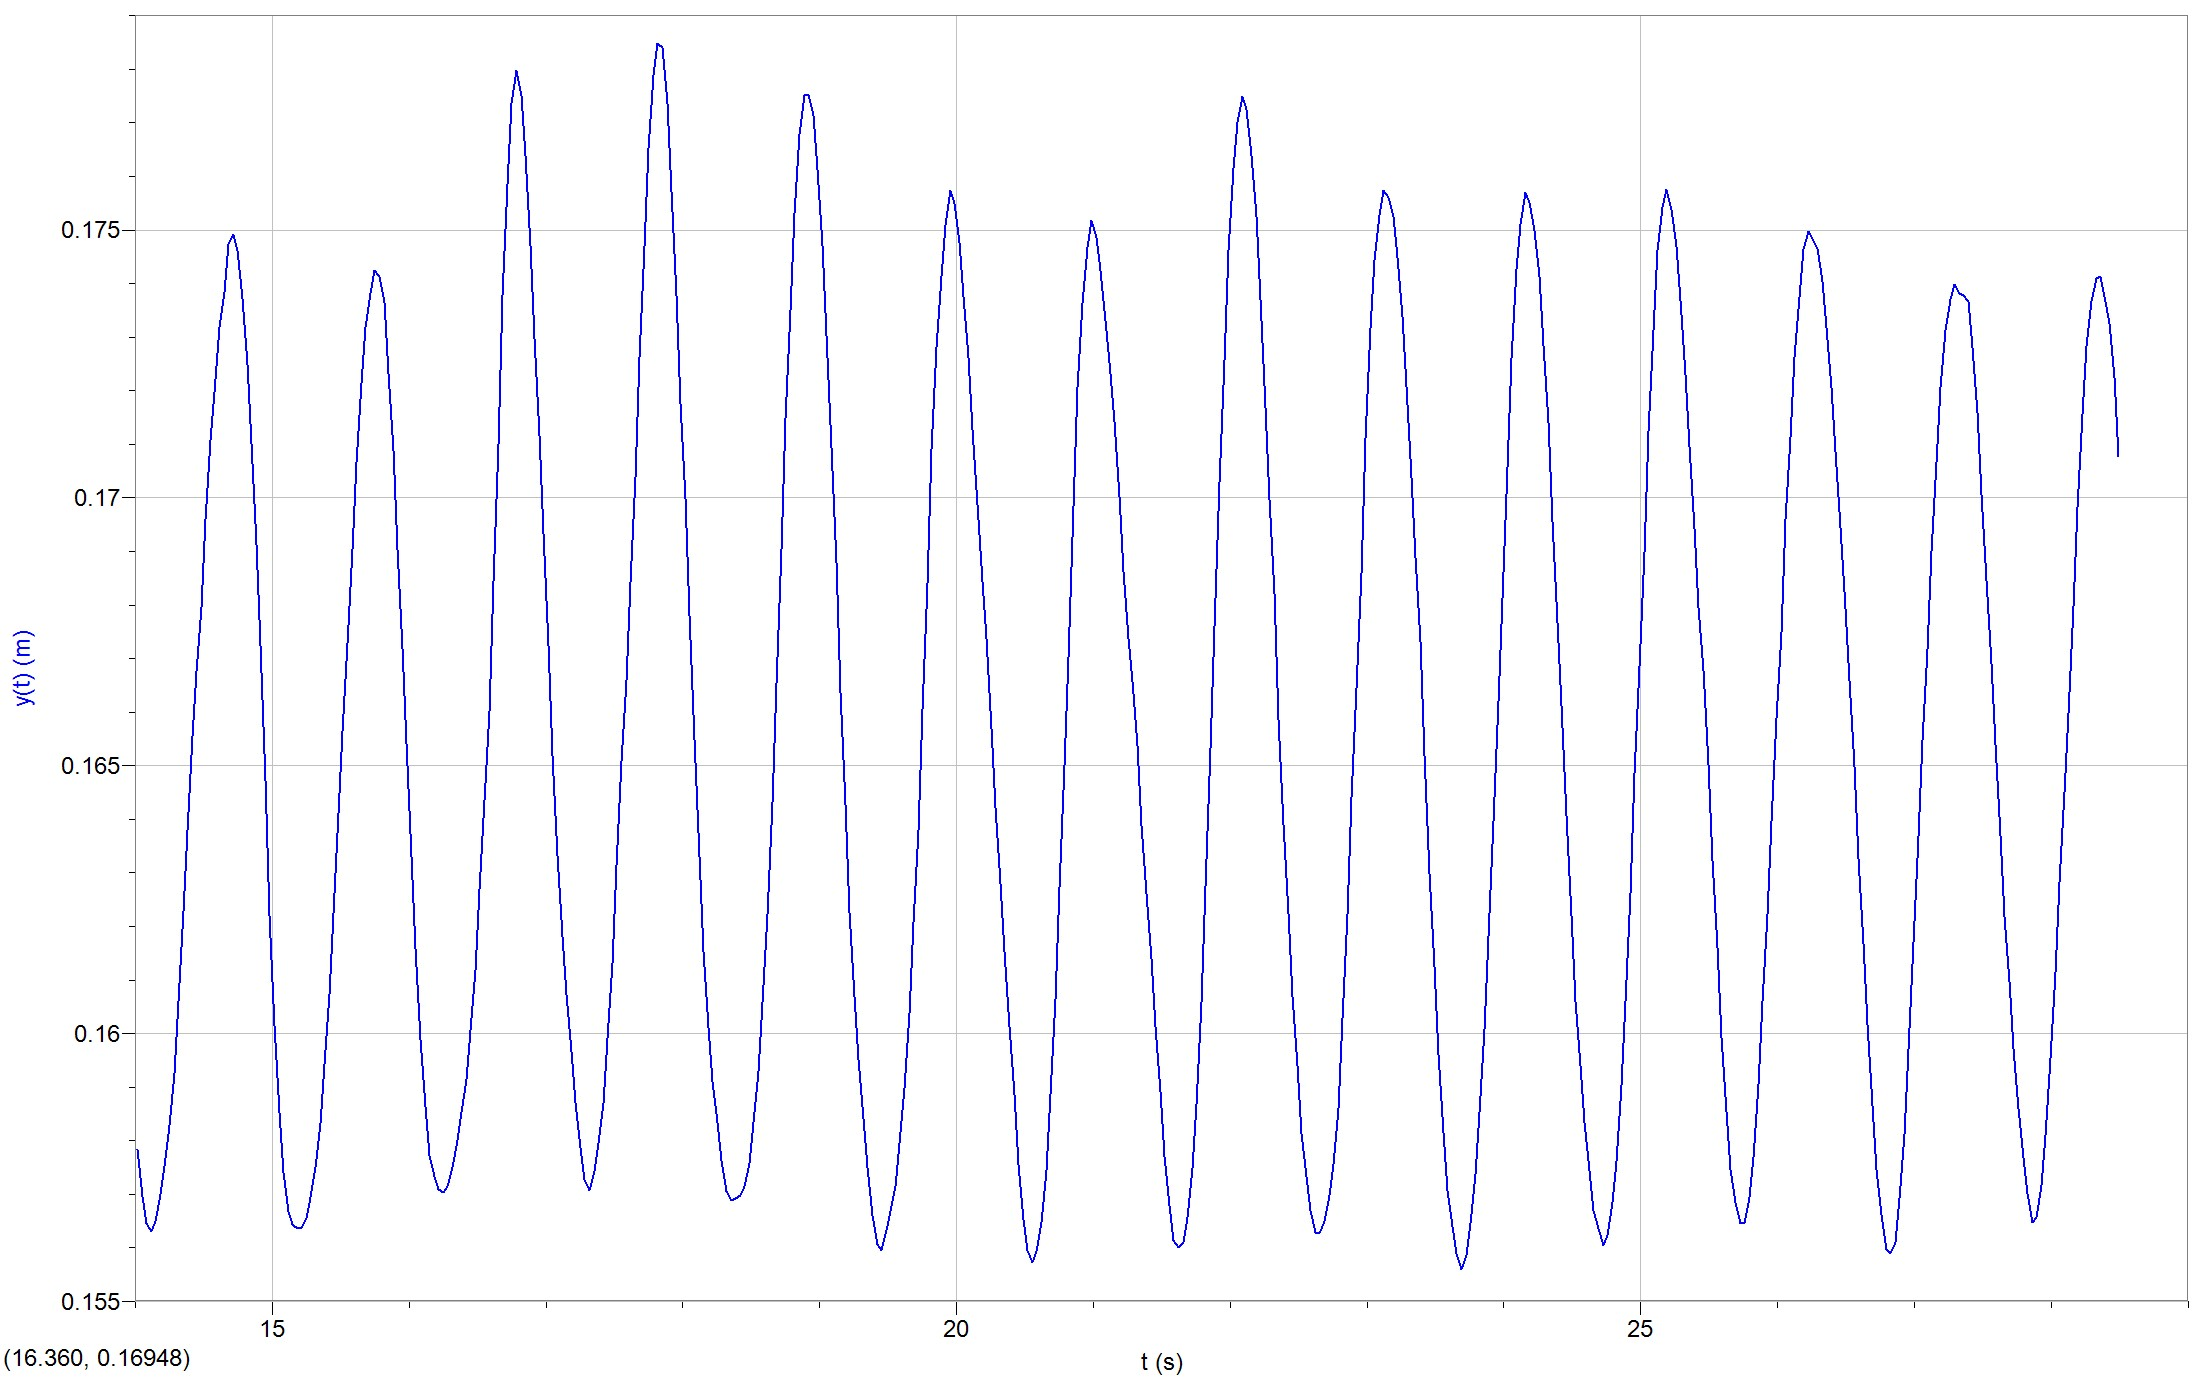
\includegraphics[width=0.70\textwidth]{images/Wave(omega=6,A=2).jpg}
    \caption{파형 데이터($A=2\mathrm{cm},~\omega=6\mathrm{rad/s}$)}
    \label{Example Wave Data}
\end{figure}

그림 \ref{Example Wave Data}는 한 sin 파의 예시이다. 코드에서는 $A=2\mathrm{cm},~\omega=6\mathrm{rad/s}$를 대입하였으며 측정값은 $A=0.9588\mathrm{cm},~\omega=5.959\mathrm{rad/s}$이다. 

\subsection{오차 원인}

본 실험에서는 실험 과정에서의 오차, 분석 상의 오차 등 여러 오차가 존재한다. 이는 크게 모터에 의한 것과 파고계 영상 분석에 의한 것으로 나눌 수 있다.

모터의 한계에 의한 것은 $\omega$에 따른 A의 한계와 아두이노에서 업로드한 파의 형태에 오차가 생기는 것이다. 최대 각가속도가 판 움직임의 진폭과 오차를 결정한다는 것은 실험을 통해 알 수 있었다. 실험은 $\omega = 6$, A = 5cm로 설정한 상태로, 각가속도만 $30,000\mathrm{step/s^2}, 40,000\mathrm{step/s^2}, 50,000\mathrm{step/s^2}$로 바꿔가며 판의 움직임을 조사하는 것으로 진행하였다. 이 때 판 움직임을 위상이 같도록 정렬한 결과가 아래의 그림이다. x축은 시간이고 y축은 판의 변위$(\mathrm{m})$이고 눈금 한 개의 스케일은 $0.01\mathrm{m}$이다.

\begin{figure}[H]
    \centering
    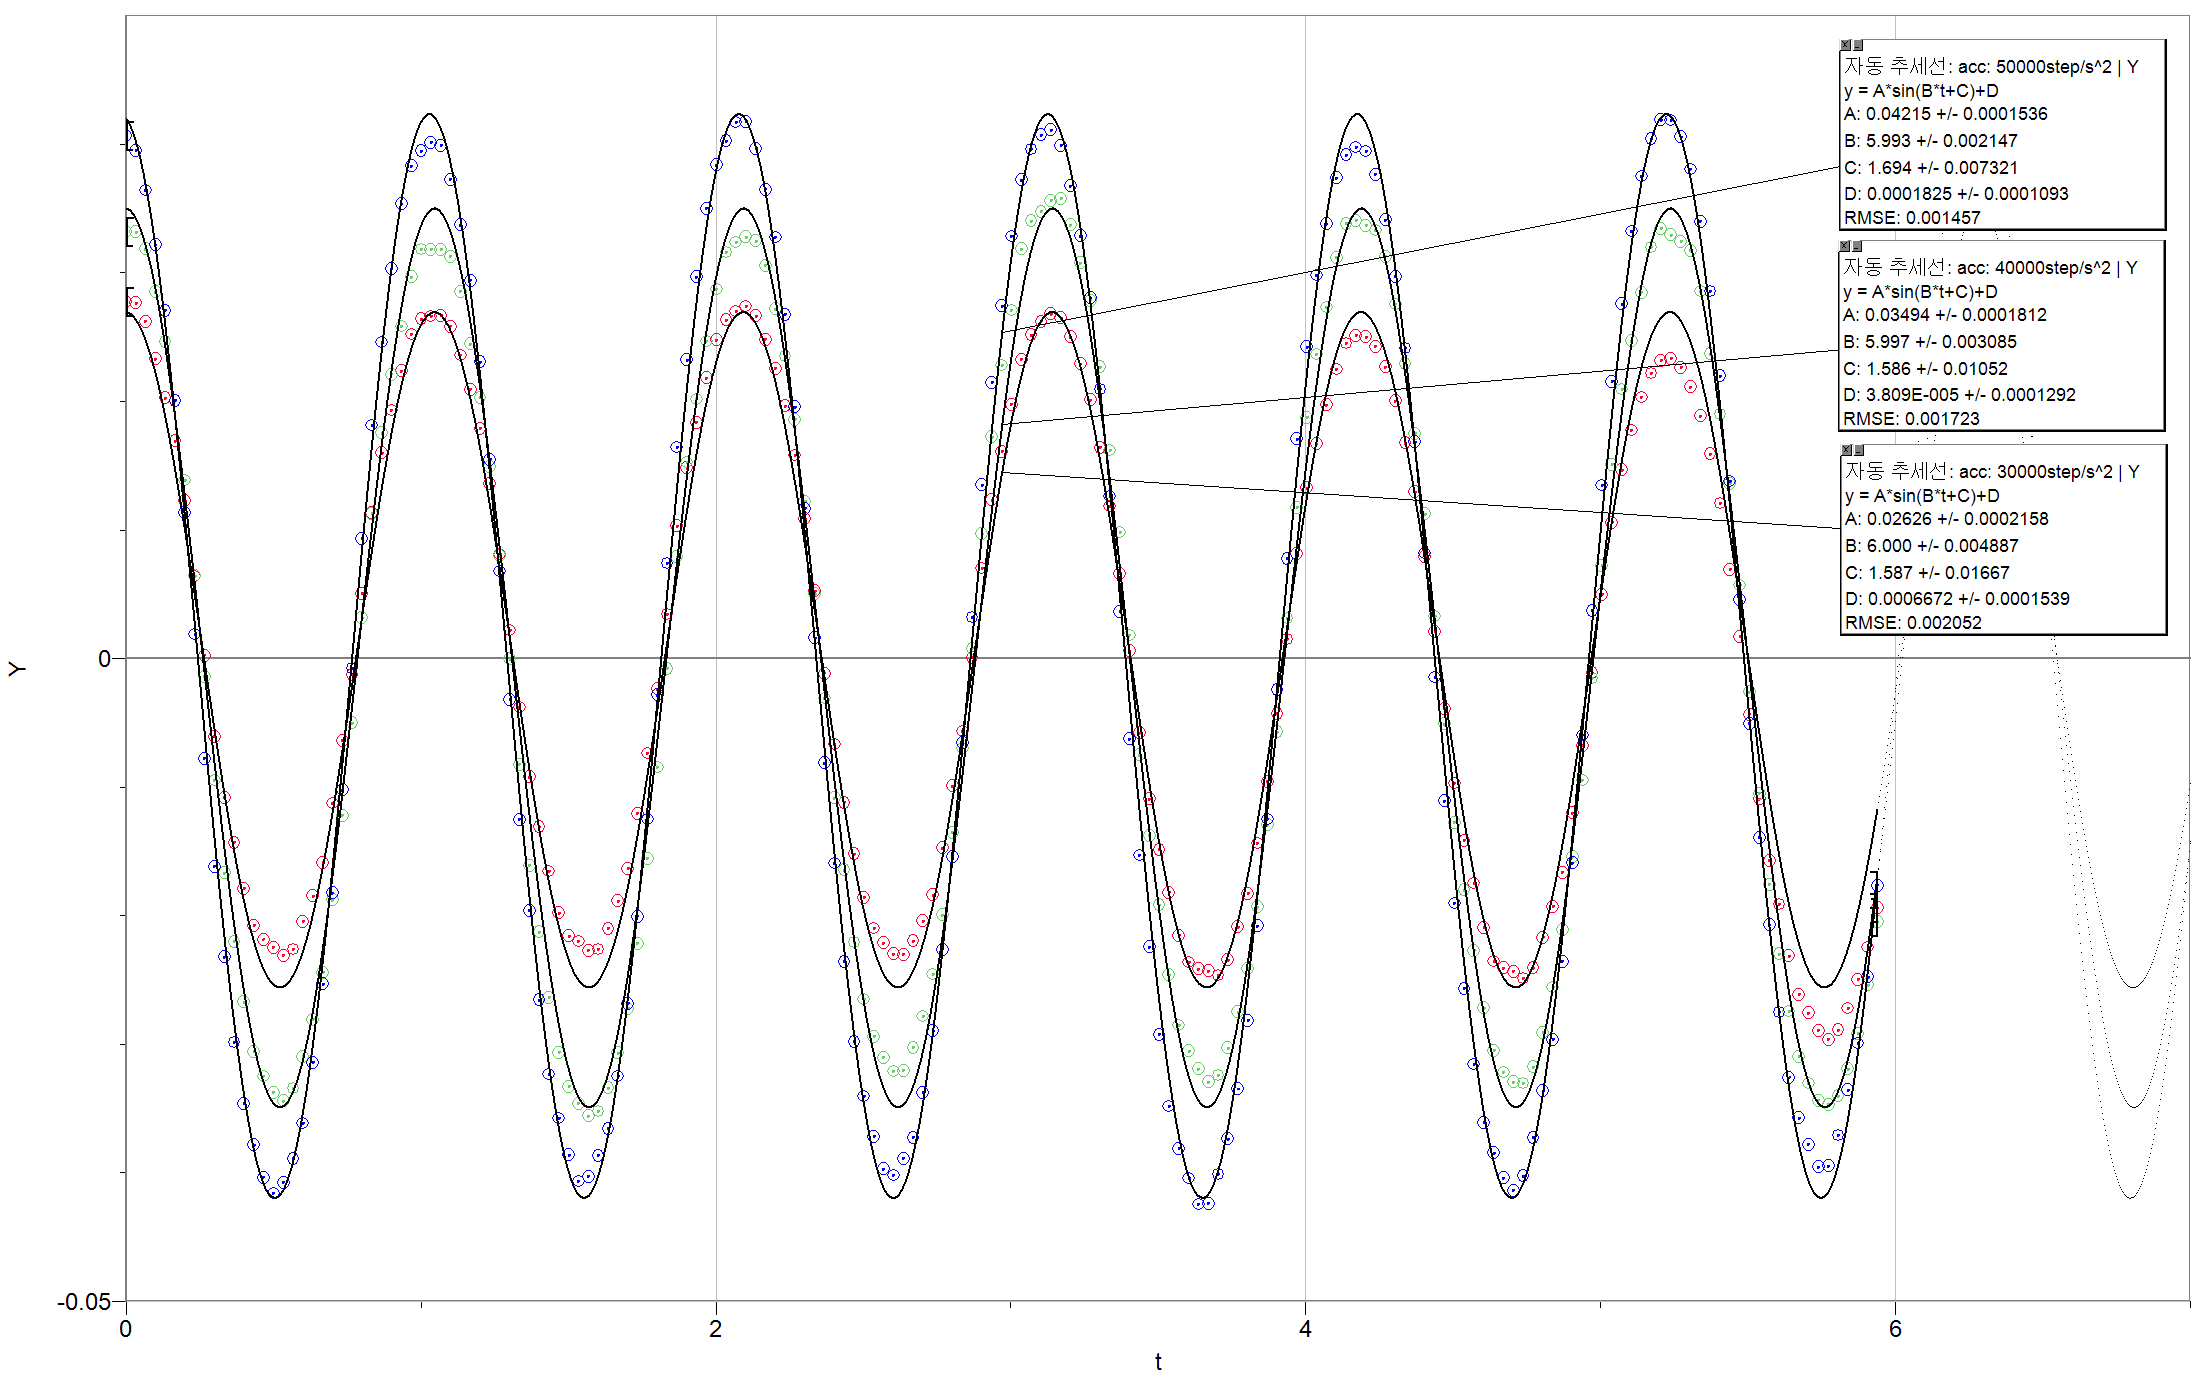
\includegraphics[width = 15cm, height = 10cm]{images/singraphofdiffacc.png}
    \caption{각가속도를 다르게 한 경우의 파고 데이터}
    \label{fig:enter-label}
\end{figure}
결과를 정리하면 각각은 다음과 같은 진폭과 진동수를 가진다.


\begin{table}[H]
    \centering
    \begin{tabular}{l|ll}
    \hline
    각가속도$(\mathrm{step/s^{2}})$ & $A (\mathrm{m})$ & RMSE \\
    \hline
    30,000 & 0.02626 & $2.052\times10^{-3}$ \\
    40,000 & 0.03494 & $1.723\times10^{-3}$ \\
    50,000 & 0.04215 & $1.457\times10^{-3}$\\
    \hline
    \end{tabular}%
\end{table}

해석하자면 목표한 진폭인 $5\mathrm{cm}$에 도달하지 못한 이유는 파의 구현에 필요한 각가속도가 $50,000\mathrm{step/s^2}$보다 크기 때문이라 볼 수 있는데, 물의 높이 $15\mathrm{cm}$를 기준으로 파가 중첩되어 생길 수 있는 최대 물의 높이에서 모터가 탈조나지 않기 위한 조건이 각가속도가 $30,000\mathrm{step/s^2}$ 이하일 것이기에 사용 중인 스텝모터로는 위의 $A-\omega$ 그래프에서 확인할 수 있는 정상적으로 구현되는 파만 구현 가능하다는 결론이 나온다.

%파도의 높낮이 변화가 극단적인 경우 부표식 파고계의 스티로폼 조각이 물 속에 잠겨버림->그로 인해서 진폭이 이론값보다 작게 나타남

%팽팽하게 위로 늘어났다가 풀리며 작은 마루가 옆에 생겨나는 현상도 관찰됨'

%쇄파 현상으로 인해 부표 위의 표식을 트래킹할 수 없

또, 본 실험에서는 스펀지와 유사한 재질의 포장재를 이용하여 얇은 직사각형판 모양의 부표를 만들었다. 이의 위치를 트래킹하여 파고를 측정하는데, 부표의 재질이 스펀지와 비슷하게 구멍이 많이 뚫려있는 재질이기에 파도의 높낮이 변화가 극단적일 경우, 물 위에 뜨지 못하고 잠시 잠기는 현상이 나타난다. 이로 인해 진폭이 이론값보다 작게 측정되는 오차가 있다. 또한 부표가 y축을 따라서만 움직이고 파도의 진행 방향에 영향을 받지 않도록 하기 위하여 부표에 두 개의 구멍을 뚫어 실을 통과시킨 후 이를 따라 움직이도록 하였는데, 마찰이 존재하므로 부표가 파도를 따라 위로 올라가는 과정에서 실이 늘어나게 된다. 실의 탄성에 의해 내려오는 과정에서 위로 튕기게 되어 파도의 큰 마루 옆에 작은 마루가 생기는 오차가 발생한다. 마지막으로, 쇄파 현상이 생기는 경우, 부표의 정중앙 표식이 부서지는 파도에 의해 가려져 정확히 같은 지점을 트래킹하는 것이 불가능하다.

%다 쓰면은 쌤한테 끝났다고 얘기하면 됨. 알겠냐? % 결과 및 토의
	%\section{결론}
\subsection{결론}

조파기는 

1. 조파기의 성능 ->
$\omega$별 정확도?
우리의 가정(진폭, 각진동수 사이 관계)은 어떻게 되었나?
됨 % 결론
        \section{추후 연구}

\subsection{실험 환경 조성}
조파기와 관련하여 여전히 많은 매개 변수와 조작 변인이 존재한다. $N$은 바꿔볼 수도 있으며 모터 드라이버의 전류나 스텝 개수를 바꿔가며 더욱 섬세한 파를 생성할 수도 있다. 이는 실험적으로 접근해야하며 시간적 제약으로 인해 제작 및 기본 실험($A,~\omega$에 따른 파 조사)만 진행하였으나 조파기에 대한 더 나은 이해가 가능하다. 파고계의 위치를 바꿔가면서 조파기와의 거리에 따른 감쇠 효과에 대해 알아볼 수도 있다.

또, 소파기에 대한 연구를 진행할 수도 있는데 현재는 바구니에 수세미를 담은 다공성 구조로 수조의 양 말단에 두었으나 이를 3D 프린터로 정형화시켜 구멍의 크기나 배치 등에 따른 소파 효과를 확인할 수도 있다. 참고문헌에 의하면 다공성 구조가 아닌 일반 벽과 같은 소파기는 표면이 포물면일 때 제일 소파 효과가 크다고 한다.


%참고문헌 필요함.

\subsection{불규칙 파 생성}
조파기의 기본적인 목표는 축소 모형 실험에서 이에 맞는 환경을 조성해주는 것으로써 불규칙 파를 생성할 수 있어야 한다. 그 방법으로는 크게 조파판을 바꾸는 방법과 파 생성함수를 바꾸는 방법이 있다. 조파판을 바꾸는 것은 일체형으로 움직이는 조파판을 여러 요소로 나누어 다르게 움직이도록 하는 것이다.

\begin{figure}[htbp]
    \centering
    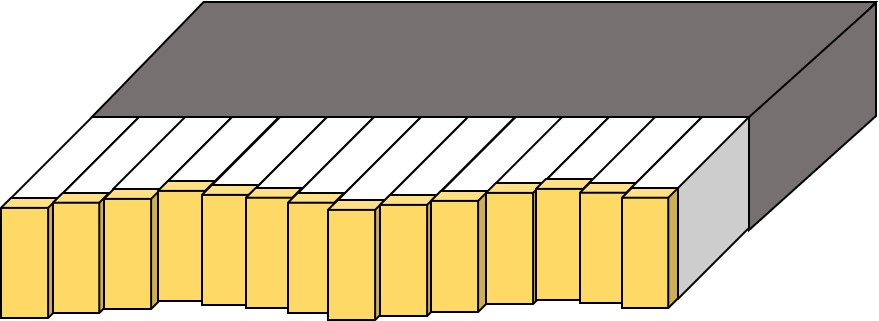
\includegraphics[width=10cm]{images/Wave_Maker(Snake).jpg}
    \caption{3차원 piston형 조파기}
    \label{Snake Wave Maker}
\end{figure}

%사진이 필요함.
이는 3차원 조파 수조로의 확장을 의미하며 조파판을 각 요소로 나누는 것이 유의미하려면 수조가 길고 좁은 것이 아닌 넓은 정사각형 모양이어야 한다. 하지만 이는 공간적 제약이 있으며 물을 여러 요소가 밀어내어 snake-like-wave를 발생시킬 수 있다. 현재는 sin파만 생성시켰으나 불규칙 파를 생성하는 것이 조파기의 궁극적인 목표이다. 그러려면 조파기가 piston형이라고 하더라도 판이 여러 조각으로 갈라져 각 조각마다 piston에 달려 있어야 하고 그만큼 많은 개수의 모터가 필요하며 아예 구동 방식을 달리 할 수도 있다. % 추후 연구
	\section{부록: Arduino Code for Wave Maker}

\subsection*{move.ino}
\begin{minted}[frame=lines, linenos, fontsize=\scriptsize]
{arduino}
void vel(int V){
  Serial.println("limitCheck");
  if(limitCheck(V)){
    float delta = V/MaxSpeed;
    delta = min(1.0f,max(-1.0f,delta));
    rotatecontrol.overrideSpeed(delta);
  }
  else vel(0);
}
boolean limitCheck(int V){
  if(analogRead(lmtPin1)<10&&V>0){
    rotatecontrol.overrideSpeed(0);
    return false;
  }
  if(analogRead(lmtPin2)<10&&V<0){
    rotatecontrol.overrideSpeed(0);
    return false;
  }
  return true;
}

void initializeMotor(){
  int V = 5000;
  while(limitCheck(V)){
    vel(V);
  }
  vel(0);
  leftEnd = motor.getPosition();
  delay(300);
  while(limitCheck(-V)){
    vel(-V);
  }
  rightEnd = motor.getPosition();
  vel(0);
  MID = (leftEnd+rightEnd)/2;
  gotoMiddle();
  Serial.println(leftEnd);
  Serial.println(rightEnd);
}
void gotoMiddle(){
    while(motor.getPosition()<MID){
      vel(5000);
    }
    vel(0);
    while(motor.getPosition()>MID){
      vel(-5000);
    }
    vel(0);
}
\end{minted}


\subsection*{sin\_wave.ino}
\begin{minted}[frame=lines, linenos, fontsize=\scriptsize]
{arduino}
int cmtostep = 400;
int A = 15;
int N = 50;
float w = 0;

void sin_set(float k,int a){
  Serial.println("sin set called");
  waveset = true;
  A = a;
  A*=400;
  w = k*PI;
   while(motor.getPosition()<MID+A){
    vel(5000);
  }
  vel(0);
  delay(5000);
  timer = 0;
  intervalTimer = 0;
}
void sinWave(){
  if(intervalTimer>N){
    intervalTimer = 0;
    float n_speed = (sinmillis(timer+N)-sinmillis(timer))/((float)N/1000);
    vel(n_speed);
    Serial.println(n_speed);
  }
}
float sinmillis(float T){
  NUM(0);
  return A*cos(w*T/1000);
}
\end{minted} % 부록
	
	\bibliography{bibfile} % 참고문헌
	% BibTeX 코드 쉽게 얻어오는 방법 %
	% Google Scholar 에서 검색한 결과에서 `인용'을 클릭한다.
	% BibTeX 코드를 얻고자 한다면, 하단의 `BibTeX' 을 클릭.
	% 코드가 나온다. Ctrl+A, Ctrl+C로 복사, bibfile에 붙여넣기.

\end{document}
